
\chapter{Conceptual Design of the 100 kW Blade using HAWTOpt2}

\section{Introduction}


\section{Aerostructural Design Tool}
\label{sec:blade_design_tool}



HawtOpt2 uses OpenMDAO v1.x \cite{openmdao} to handle the definition of the optimization problem, workflow, dataflow and parallelization of simulation cases.
This allows us to efficiently make use of high performance computing clusters, with MPI parallelisation of both cases within the objective function (e.g. design load cases), as well as the evaluation of finite difference gradients.
OpenMDAO provides an interface to PyOptSparse~\cite{pyopt} which has wrappers for several optimization algorithms.
In this work, the open source gradient-based interior point optimizer IPOPT \cite{ipopt} is used. 
HawtOpt2 has interfaces to the finite element cross sectional tool BECAS~\cite{blasquesb, becas} and to the aeroelastic tools HAWC2~\cite{hawc2_manual} and HAWCStab2~\cite{hansen_aeroelastic_2004}. 
BECAS allows for the evaluation of the cross sectional structural and mass properties of the blade, as well as calculation of material failure both with respect to ultimate and fatigue loads.
HAWCStab2 uses an unsteady blade element momentum (BEM) model of the rotor and a geometrically non-linear finite beam element model to compute steady-state aerodynamic states, structural deflections and linearized models of the wind turbine. 
HAWCStab2 has an analytical linearisation of the high-order aeroservoelastic model, which can be used for frequency analysis, controller tuning and evaluation of fatigue damage equivalent load rates using a frequency domain based approach \cite{tibaldi2015}. 
Untimate loads simulations within the optimization loop are carried out using the aero-hydro-servo-elastic software package HAWC2 on a reduced set of design load cases as per IEC 61400-1 Ed3, while the final designs are evaluated using the full design load basis described in ref. \cite{hansen2015}.

Figure~\ref{fig:xdsm} shows a so-called extended design structure matrix diagram (XDSM)~\cite{Lambe2012} of the workflow in HawtOpt2.
Overlaid boxes indicate components that are executed in parallel for each cross-section/load case.
At the upper level, the entire workflow is parallelised to enable parallel gradient evaluation.
All of these parallelisations are embarrassingly parallel and thus this scales linearly with the number of CPUs available.
A typical optimization will use 20 cores per objective function evaluation, and be parallelised according to the available resource with $n$ number of concurrent FD gradient evaluations.
For the present study 30 concurrent FD evaluations were used. A single objective evaluation required approximately 4 minutes, and therefore approximately 12 minutes per major iteration for 60 design variables, using a total of 600 cores.\footnote{Parts of the text above describing the tools used and the overall optimization framework are excerpts from Zahle et al \cite{zahle2016}. Refer to this article for a full description of the tools and most recent results.}

\begin{figure}[!ht]
\begin{center}
	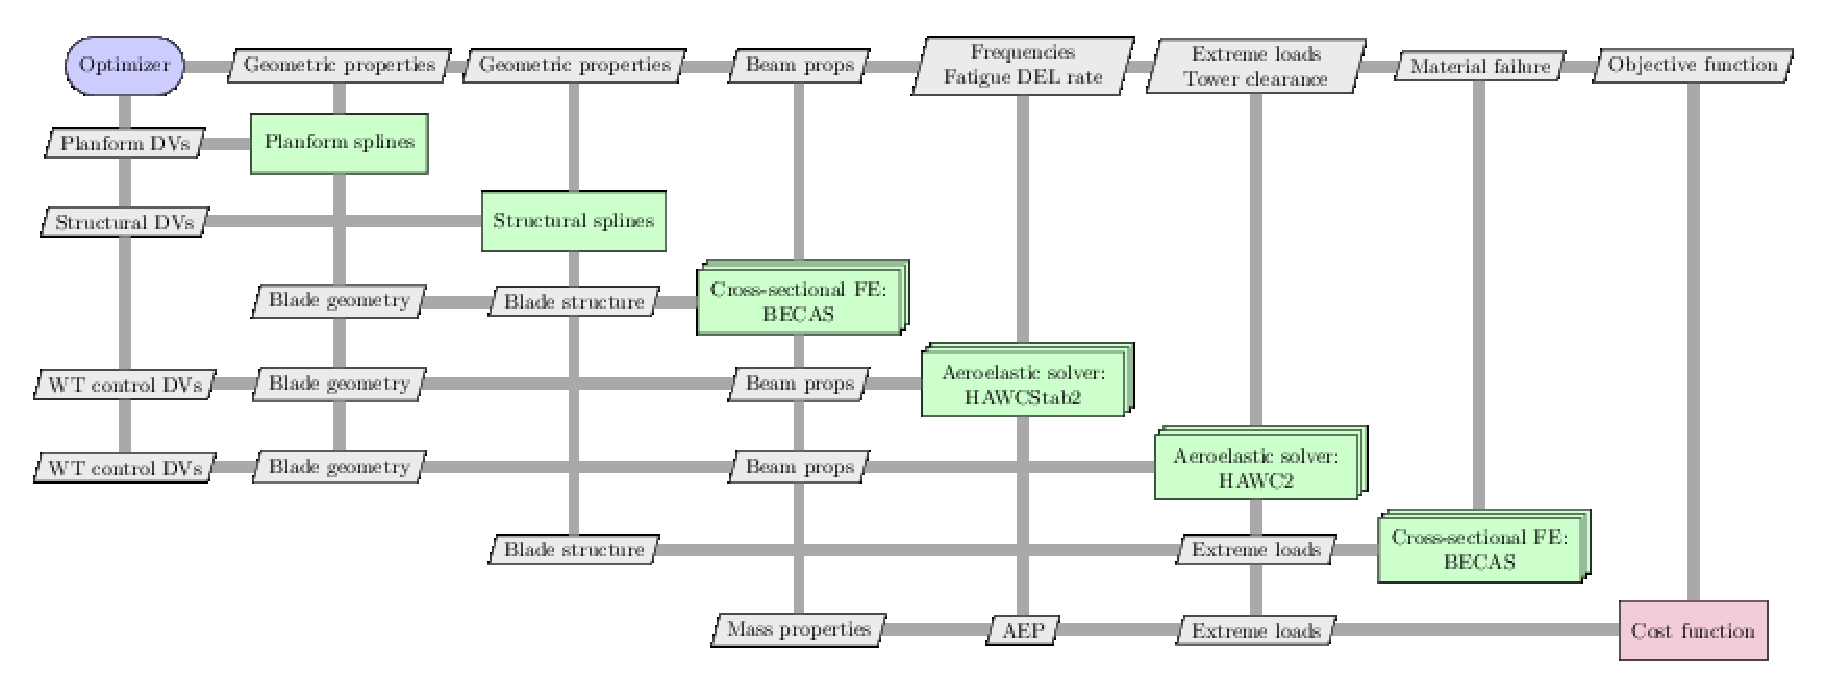
\includegraphics[width=1\linewidth]{figures/hawtopt2_xdsm.eps}
\end{center}
\caption{Extended Design Structure Matrix diagram of the workflow of HawtOpt2.}
\label{fig:xdsm}
\end{figure}


\section{Blade Paramerization}
\label{sec:blade_params}

The blade planform is described in terms of distributions of chord, twist, relative thickness and pitch axis aft leading edge, the latter being the distance between the leading edge and the blade axis.
The lofted shape of the blade is generated based on interpolation of a family of airfoils with different relative thicknesses.

The internal structure is defined from a number of regions that each cover a fraction of the cross-sections along the blade.
Each region consists of a number of materials that are placed according to a certain stacking sequence.
Figure~\ref{fig:cross_section_def} shows a cross section in which the region division points (DPs) are indicated along with the parameterized quantities used to construct the structural geometry.
The composite layup is described by a series of smooth splines describing the thicknesses of individual layers. 
Fore more details on the parameterisation see \cite{fusedwind}.

\begin{figure}[!ht]
\begin{center}
        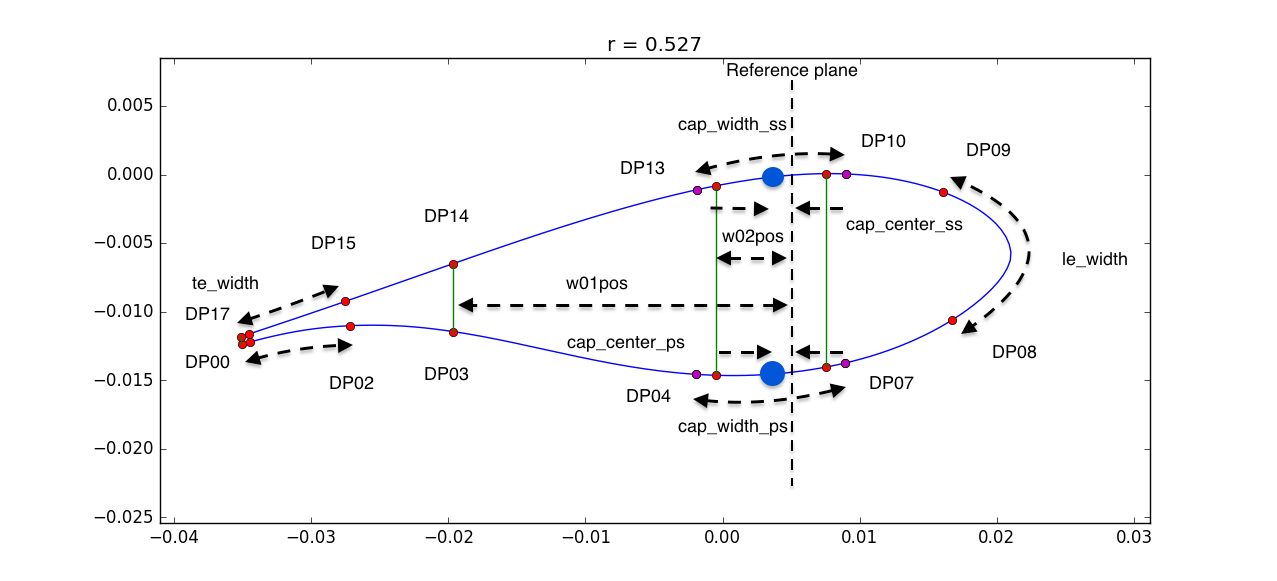
\includegraphics[width=1.\linewidth]{./figures/param2_schematic.eps}
\end{center}
\caption{Region division points (DP) definition: red points indicate division points between regions; their positions are defined as curve fraction from pressure side TE (s=-1) to LE (s=0) to suction side TE (s=1).}
\label{fig:cross_section_def}
\end{figure}

\section{Baseline Design}

The initial data supplied to the project regarding the 100 kW blade consisted of stiffness data as well blade planform, and overall operational characteristics, and component masses.
Data on the airfoils used on the blades or their performance were not supplied.
Neither were details on the internal structure and the materials used.

Several choices had to be made during the initial phases.
In the bullet list below the main choices are listed:

\begin{itemize}

	\item Airfoils: The main airfoil series used is the FFA-W3 series along with a NACA-63-418 tip airfoil.
	\item Airfoil data: Airfoil data was computed using the 2D incompressible CFD solver EllipSys2D \cite{michelsen92,michelsen94,sorensen95}, as a 70/30 blend of clean and tripped flow conditions computed at $Re=1\times10^6$.
	\item Materials: The blade consists of glass fibre only. Materials used are the same as on the DTU 10MW RWT \cite{bakrwt}.
	\item Structural layout: Conventional box structure with linearly tapered main laminates connected with two shear webs.
	\item Blade planform: Based on the externally supplied planform.
\end{itemize}


The following sub-sections describe the steps taken to design the fully described aerostructural blade design for the 100 kW rotor.

\subsection{Airfoil series}

The main airfoil series used is the FFA-W3 series along with a NACA-63-418 tip airfoil.
Figure \ref{fig:baseline_airfoils} shows the 2D cross-sectional shapes of these airfoils.
Figures \ref{fig:baseline_cl} to \ref{fig:baseline_LD} show the lift, drag and lift-to-drag polars of the airfoils computed at a Reynolds number of $Re=1\times10^6$ using EllipSys2D with a mesh consisting of 512 cells in the chordwise direction and 192 cells in the normal direction.
To account for effects of roughness, the polars used were generated from a blend of clean surface, free transition flow and fully turbulent flow, with a blend factor of 0.7/0.3.
360 degree extrapolation of the airfoil data was done using the Viterna method.\footnote{http://wisdem.github.io/AirfoilPreppy/} No 3D correction of the airfoil data was done since the position of the airfoils are changed during optimization, making the 3D correction invalid since it depends on the spanwise position.

\begin{figure}[!ht]
\begin{center}
	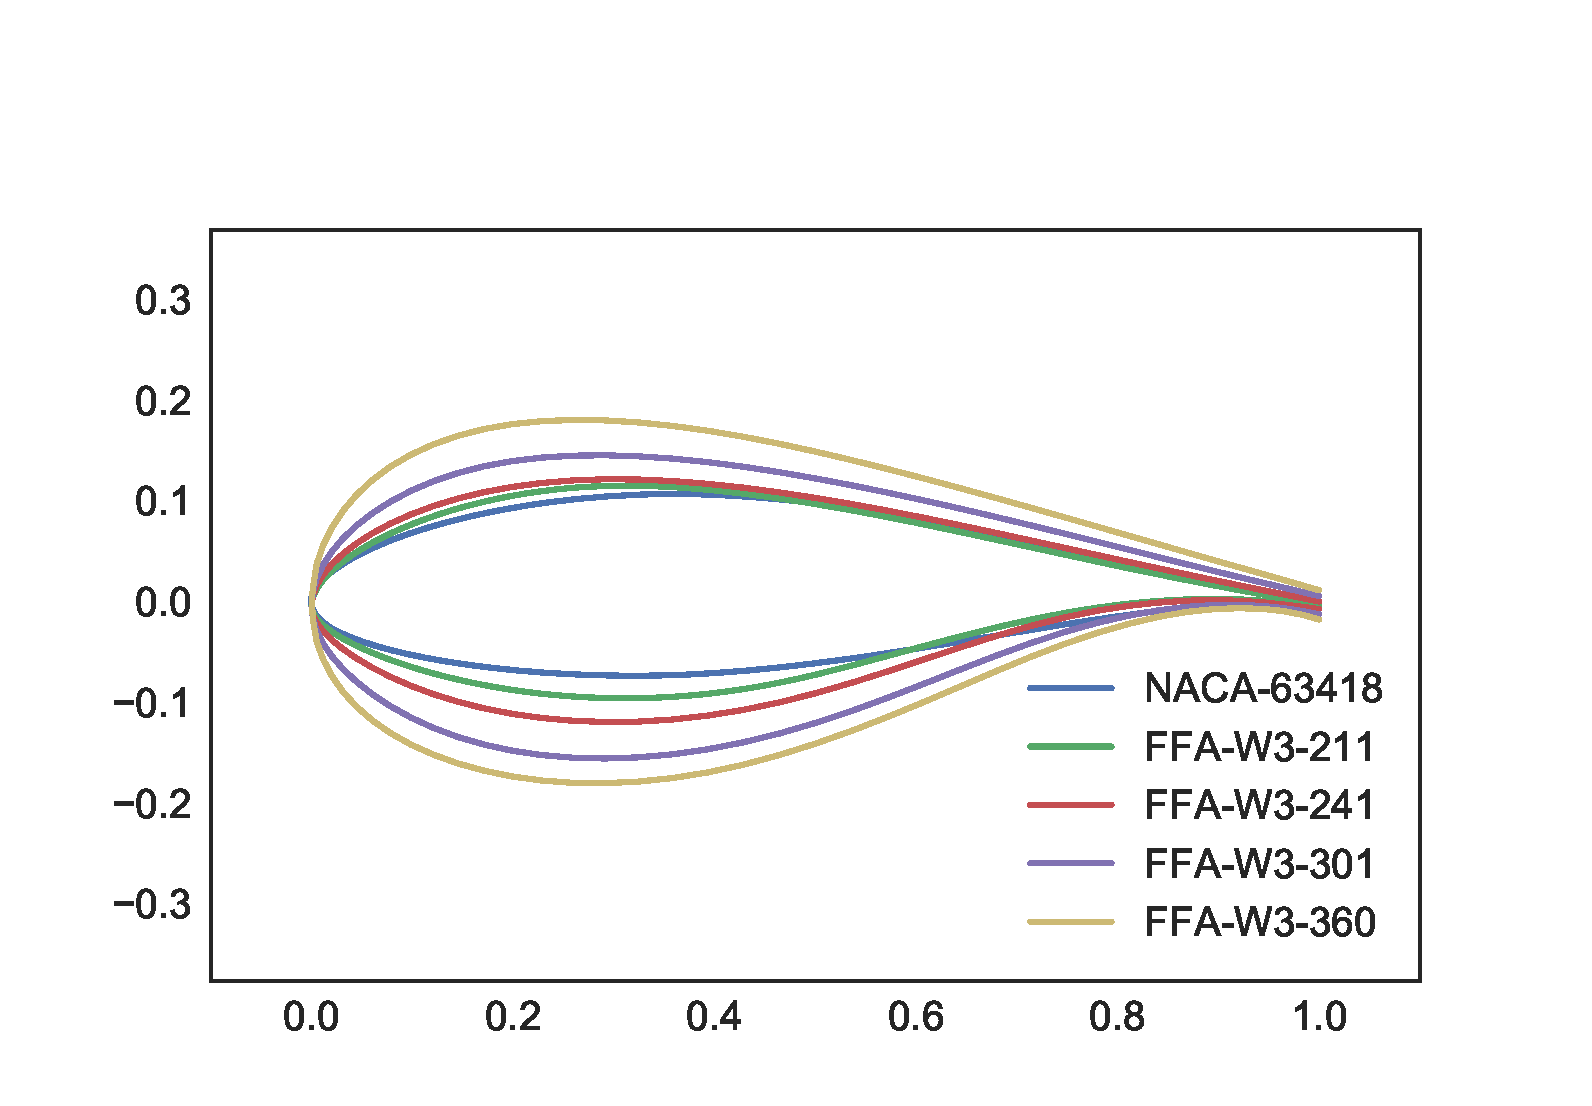
\includegraphics[width=0.8\linewidth]{figures/KB_airfoil_series.eps}
\end{center}
\caption{Airfoils used on the 100kW baseline blade.}
\label{fig:baseline_airfoils}
\end{figure}

\begin{figure}[!ht]
\begin{center}
	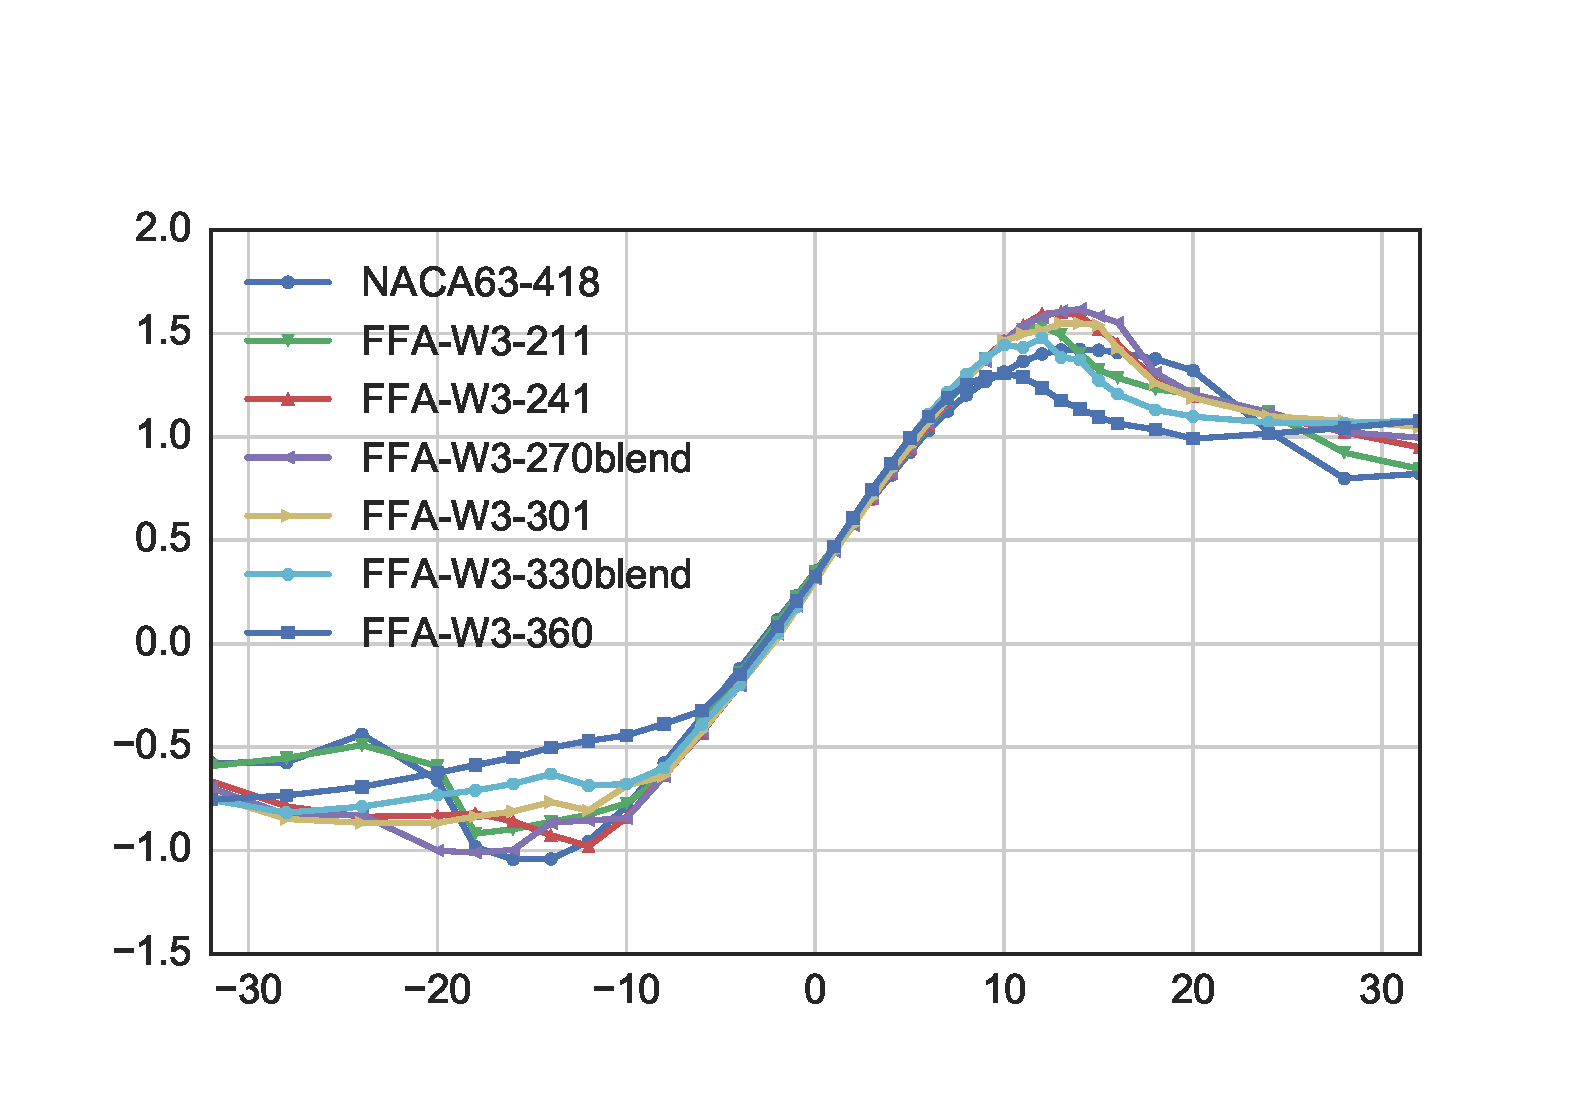
\includegraphics[width=0.8\linewidth]{figures/KB_airfoil_data_cl_detail.eps}
\end{center}
\caption{Airfoil lift coeffients as function of AOA computed at $Re=1e6$.}
\label{fig:baseline_cl}
\end{figure}

\begin{figure}[!ht]
\begin{center}
	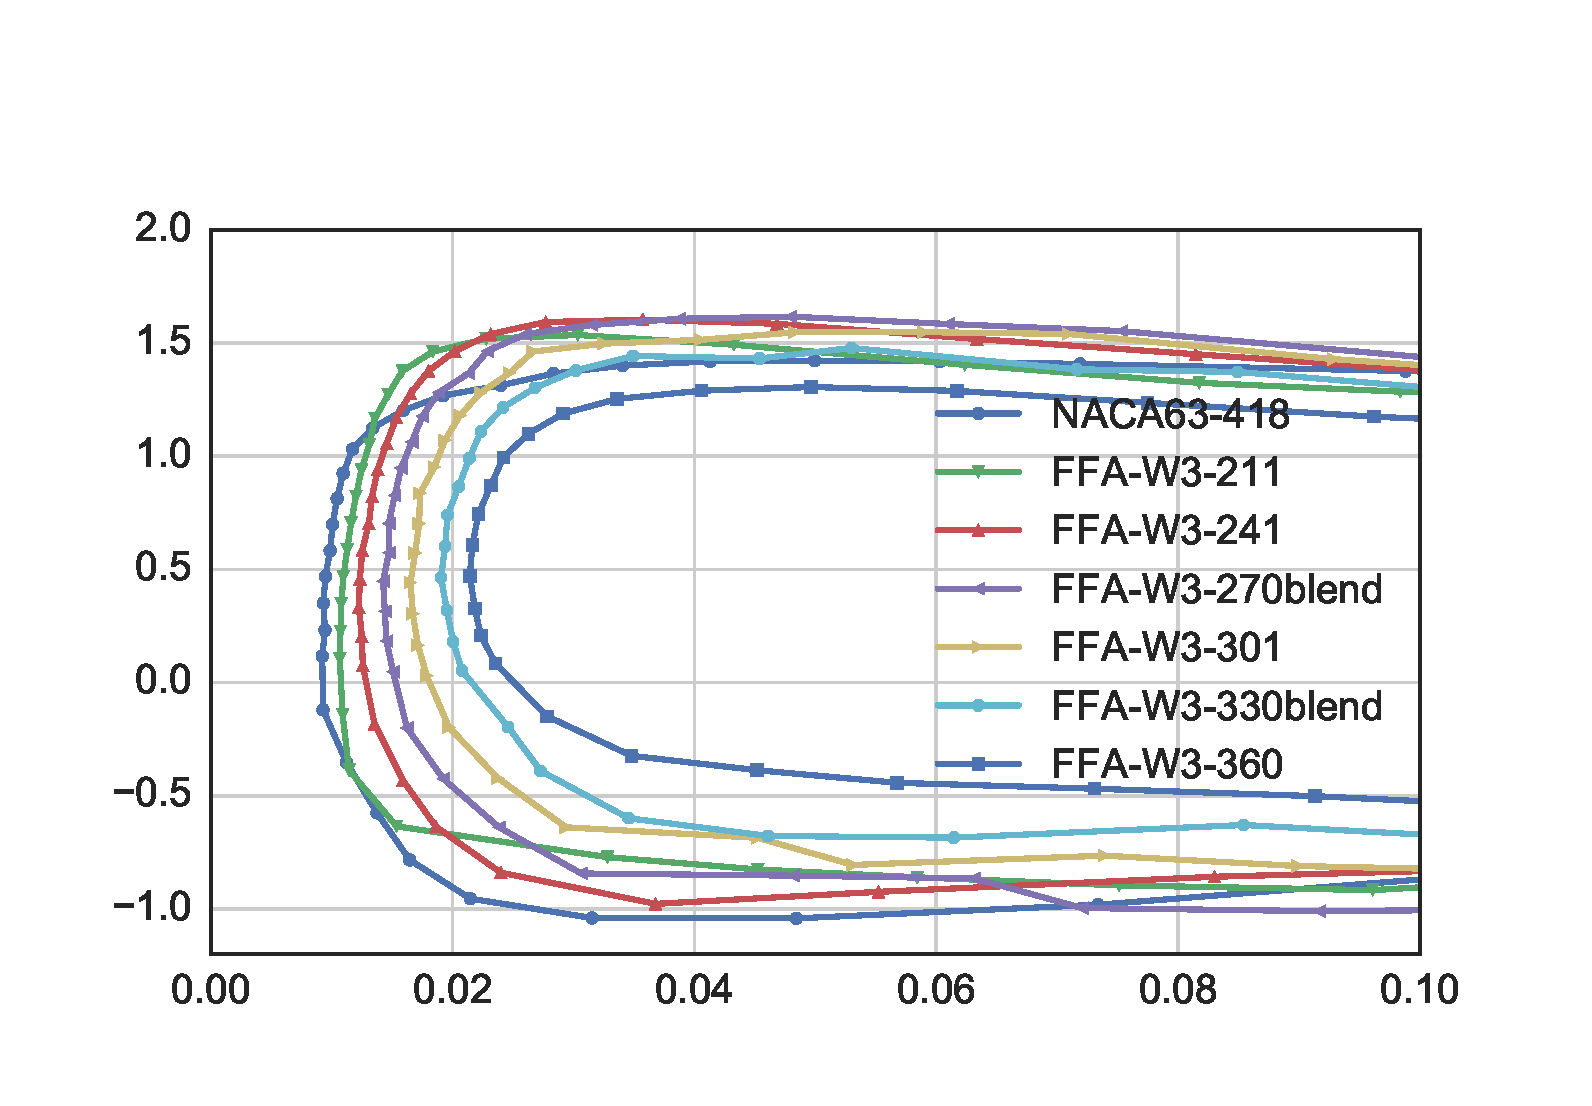
\includegraphics[width=0.8\linewidth]{figures/KB_airfoil_data_cd_detail.eps}
\end{center}
\caption{Airfoil drag coeffients as function of AOA computed at $Re=1e6$.}
\label{fig:baseline_cd}
\end{figure}

\begin{figure}[!ht]
\begin{center}
	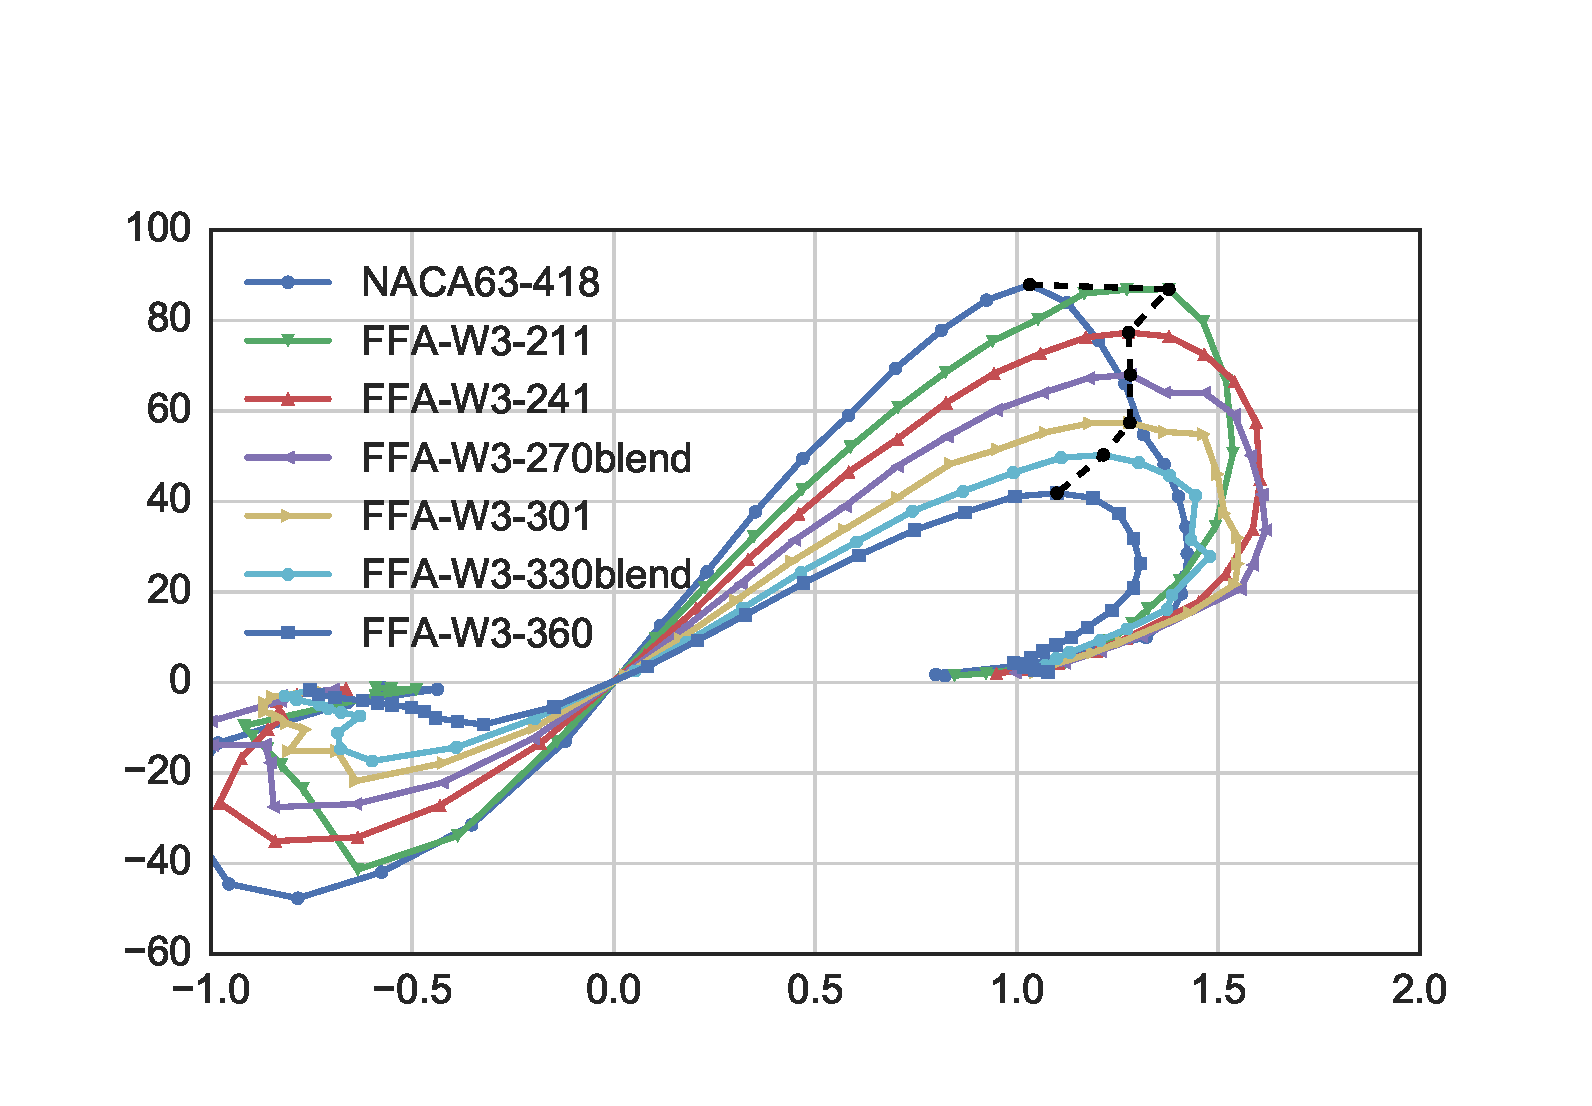
\includegraphics[width=0.8\linewidth]{figures/KB_airfoil_data_clcd_detail.eps}
\end{center}
\caption{Airfoil lift to drag ration as function of $C_l$ computed at $Re=1e6$.}
\label{fig:baseline_LD}
\end{figure}

\clearpage

\subsection{Reference Materials}
\label{sec:reference_mats}

The material properties used for the blade where those defined for the DTU 10 MW RWT (for more details, see \cite{dtu10mwrwt}).
Table \ref{tab:robi_matprop_laminates} lists the apparent mechanical properties of the multidirectional plies used. 

\begin{table}[h!]
\setlength\extrarowheight{2pt}
\centering
\begin{threeparttable}
\begin{tabular}{lcccc}
Multidirectional Ply    &  \multicolumn{1}{c}{Uniax}  &  \multicolumn{1}{c}{Biax}  & \multicolumn{1}{c}{Triax}  & \tabularnewline
\hline
Fiber volume fraction  $V_\text{f}$   &  0.55  &  0.5  &  0.5  &  -        \tabularnewline
Unidirectional lamina  & \multicolumn{1}{c}{Lamina 2} & \multicolumn{1}{c}{Lamina 1}    & \multicolumn{1}{c}{Lamina 1} & \tabularnewline
\hline
\ang{0} fibers                        &  95    &  0    &  30   & \%  \tabularnewline
\ang{90} fibers                       &  5     &  0    &  0    & \%  \tabularnewline
\ang[retain-explicit-plus]{+45} fibers                       &  0     &  50   &  35   & \%  \tabularnewline
\ang{-45} fibers                      &  0     &  50   &  35   & \%  \tabularnewline
\hline
Young's modulus      $E_1$            &  41.63   & 13.92   &   21.79  & GPa      \tabularnewline
Young's modulus      $E_2$            &  14.93   & 13.92   &   14.67  & GPa      \tabularnewline
Shear modulus     $G_{12}$            &  5.047   & 11.50   &   9.413  & GPa      \tabularnewline
Poisson's ratio $\nu_{12}$            &  0.241   & 0.533   &   0.478  & -        \tabularnewline
Shear modulus $G_{13}=G_{23}$\tnote{(a)} &  5.04698 & 4.53864 &  4.53864 & GPa      \tabularnewline
Mass density        $\rho$            &  1915.5  & 1845.0  &  1845.0  &  $kg/m^3$  \tabularnewline
\hline
\end{tabular}
%\begin{tablenotes}
%\item [(a)] not computed but chosen identical to the values of the respective laminae in Table~\ref{tab:robi_matprop_laminae}.
%\end{tablenotes}
\end{threeparttable}
\caption{Fiber orientation and apparent mechanical properties of the multidirectional plies.}
\label{tab:robi_matprop_laminates}
\end{table}

Design strength properties are also defined for these materials\footnote{Internal communication, provided by Peter Berring} and are listed in Table \ref{tab:matprops_strength}.

\begin{table}[h!]
\setlength\extrarowheight{2pt}
\centering
\begin{tabular}{lccccccccc}
\hline
\hline
	&$\sigma_{11}^t$ & $\sigma_{22}^t$  & $\sigma_{33}^t$  & $\sigma_{11}^c$  & $\sigma_{22}^c$  & $\sigma_{33}^c$  & $\tau_{12}$   & $\tau_{13}$   & $\tau_{23}$     \\
\hline
Biax	&	69.3         & 69.3  & 69.3  &  64.9 & 64.9  & 64.9  & 55.9 & 55.9 & 55.9 \\
Uniax	&	 360.0         & 24.8  & 24.8  & 257.0 & 63.5  & 63.5  & 16.6 & 16.6 & 16.6  \\
Balsa 	&	 1.0         &  1.0  &  1.0  &   1.0 &  1.0  &  1.0  &  1.0 &  1.0 &  1.0 \\
Triax 	&	186.0         & 30.5  & 30.5  & 152.0 & 51.5  & 51.5  & 42.3 & 42.3 & 42.3 \\
\hline
\hline
\end{tabular}
\caption{Design strength properties of the multidirectional plies.}
\label{tab:matprops_strength}
\end{table}


\begin{table}[h!]
\setlength\extrarowheight{2pt}
\centering
\begin{tabular}{lccccccccc}
\hline
\hline
	&$\epsilon_{11}^t$     & $\epsilon_{22}^t$ & $\epsilon_{33}^t$ & $\epsilon_{11}^c $   & $\epsilon_{22}^c$ & $\epsilon_{33}^t$ & $\gamma_{12}$    & $\gamma_{13} $    & $\gamma_{23}$     \\
\hline
Biax	&	 6.802e-3 & 1.0e6 & 1.0e6 & 7.255e-3 & 1.0e6 & 1.0e6 & 1.0e11 & 1.0e+11 & 1.0e+11 \\
Uniax	&	 6.802e-3 & 1.0e6 & 1.0e6 & 9.523e-3 & 1.0e6 & 1.0e6 & 1.0e11 & 1.0e+11 & 1.0e+11 \\
Balsa 	&	1.000e+6 & 1.0e6 & 1.0e6 & 1.000e+6 & 1.0e6 & 1.0e6 & 1.0e11 & 1.0e+11 & 1.0e+11 \\
Triax 	&	 8.162e-3 & 1.0e6 & 1.0e6 & 9.976e-3 & 1.0e6 & 1.0e6 & 1.0e11 & 1.0e+11 & 1.0e+11 \\
\hline
\hline
\end{tabular}
\caption{Design strength properties of the multidirectional plies.}
\label{tab:matprops_strength}
\end{table}

\clearpage

\subsection{Structural Layout}
\label{sec:sizing}

An approximate sizing of the internal structure was carried out in order to match the stiffness properties supplied from the external partners.
This was done using the BECAS interface in HAWTOpt2, where material thickness distributions in 19 cross-sections along the span were sized to match flapwise stiffness, $EI_x$, edgewise stiffness, $EI_y$, and torsional stiffness, $GJ$.
Following this optimization, the material thicknesses were adjusted manually to obtain a reasonably smooth material distribution along the blade.

Table \ref{tab:structure_props} shows the overall properties of the structural geometry. 
The spar cap was tapered from a width of 0.2 m at the root to 0.1 m at the tip, and the trailing edge and leading edge reinforcements had a width of 0.08 and 0.12 m, respectively.
The structural geometry for the blade is plotted in Figure \ref{fig:loftedstructure_baseline_tipview}.

\begin{table}[h!]
\centering
\small
\begin{tabular}{{ll}}
\hline
	Spar cap widths	 						& Linear taper 0.2 m (root) to 0.1 m (tip) \\
	Trailing edge panel width upper			& 0.08 m	\\
	Trailing edge panel width lower			& 0.08 m	\\
	Leading edge panel width (upper+lower)	& 0.12 m \\
	Shear web angle relative to rotor plane	& 90 deg	\\
\hline
\end{tabular}
\caption{Overall properties of internal structure.}
\label{tab:structure_props}
\end{table}


\begin{figure}[!ht]
\begin{center}
	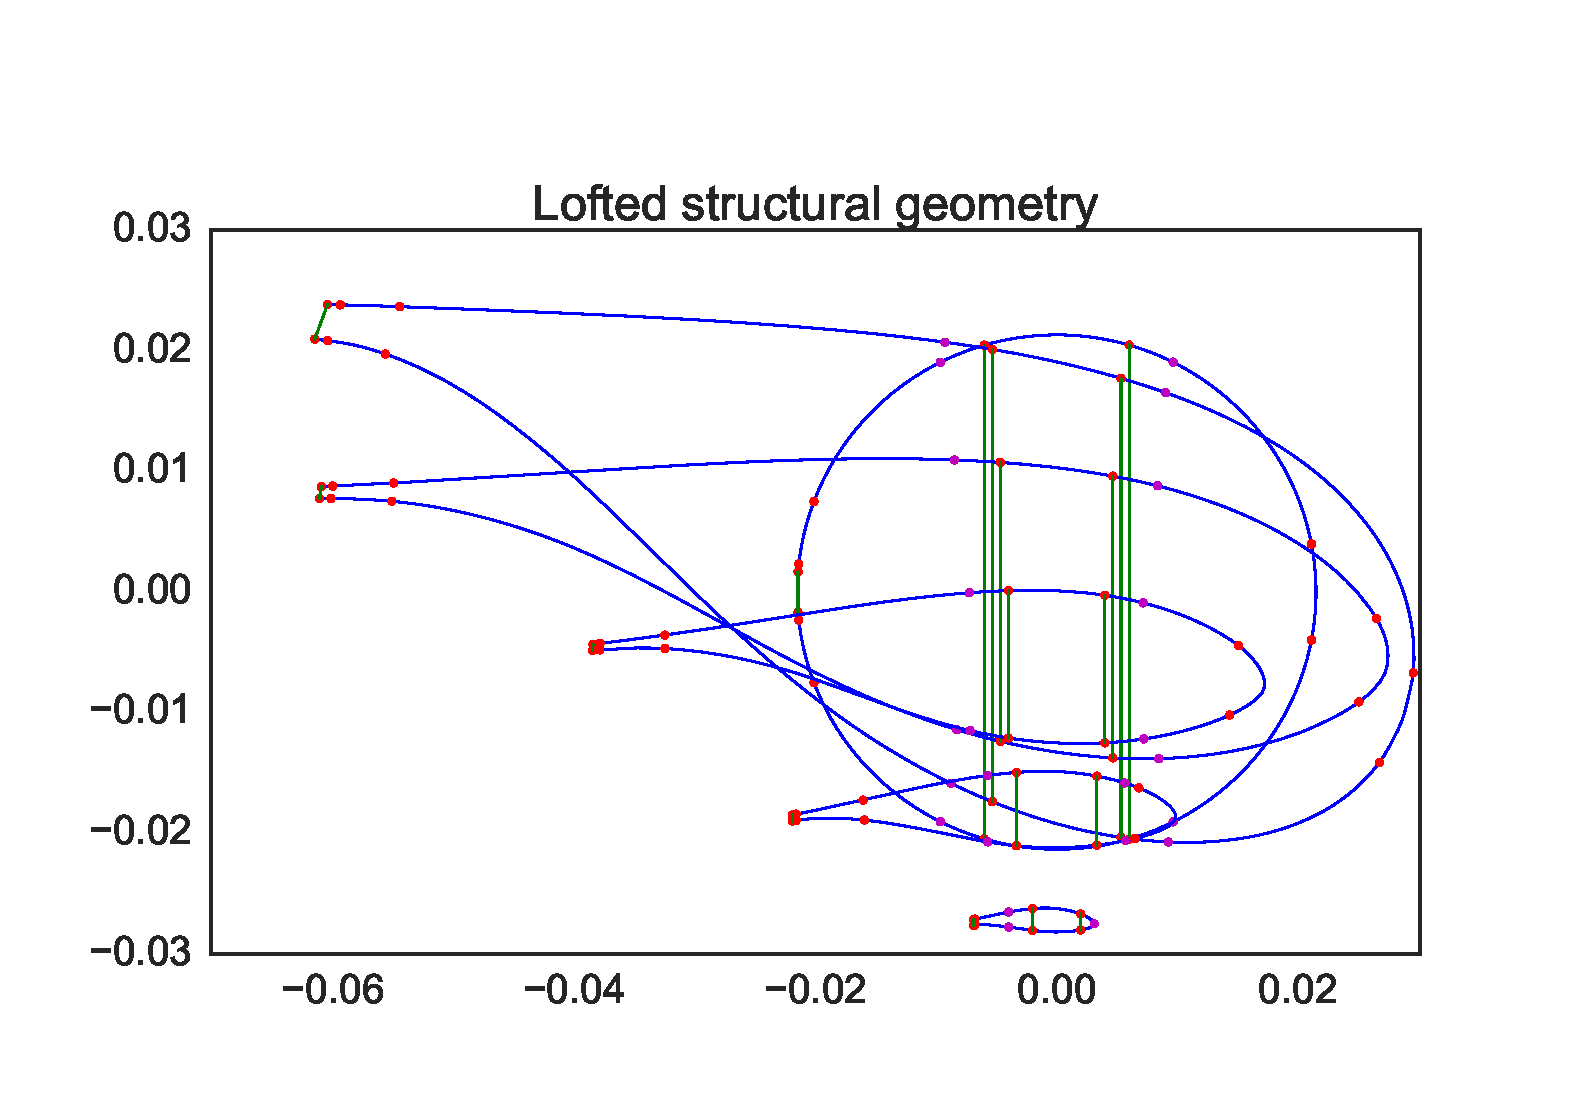
\includegraphics[width=1\linewidth]{figures/baseline_blade_tipview.eps}
\end{center}
\caption{Lofted blade showing internal structural geometry.}
\label{fig:loftedstructure_baseline_tipview}
\end{figure}

Figure \ref{fig:loftedstructure_baseline} shows a 3D plot of the lofted blade structure with material distributions.
Figure \ref{fig:layups} shows the detailed stacking sequence of materials in the blade.
The total mass of the blade resulting from the sizing process was approximately 230 kg.
This does not include adhesives, surface finishing, and a complete root design.

\begin{figure}[!ht]
\begin{center}
	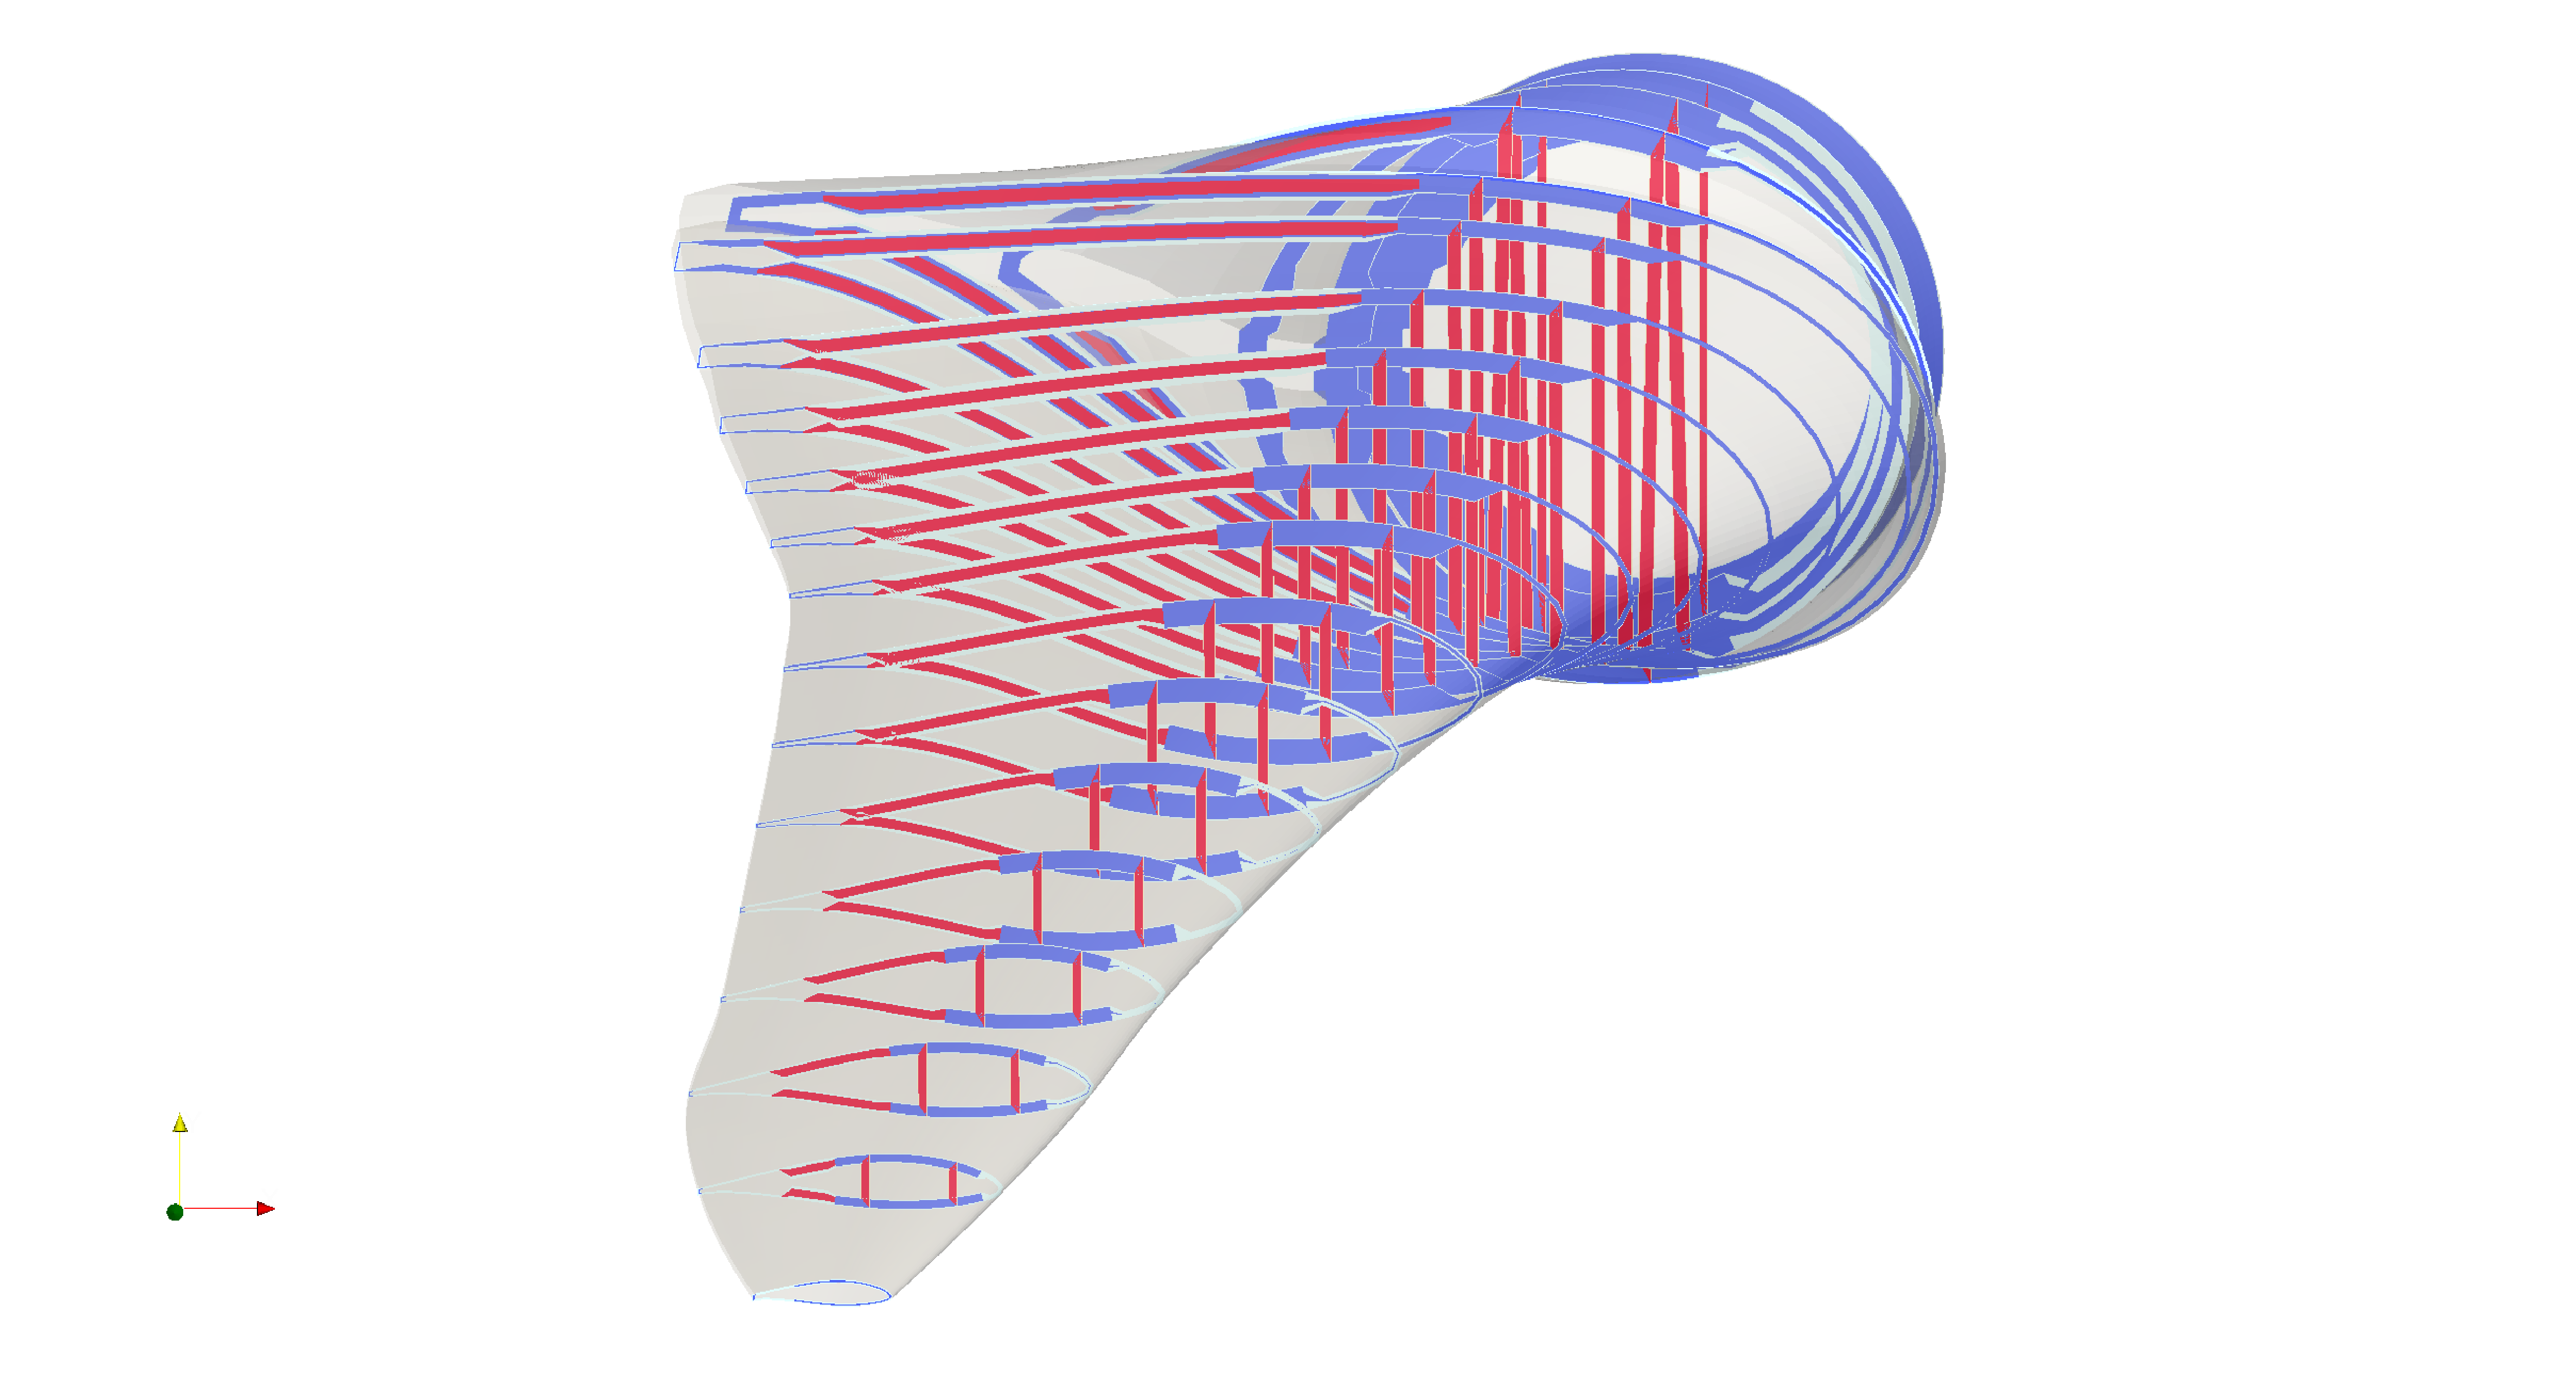
\includegraphics[width=1\linewidth]{figures/loftedbladestructure_basic_sizing.eps}
\end{center}
\caption{Lofted blade showing internal structural geometry.}
\label{fig:loftedstructure_baseline}
\end{figure}

\clearpage
%%------------------------------------------------------------------------------------------------------
%% Start of design compariosions from HAWTOpt2
%%-----------------------------------------------------------------------------------------------------
\section{Design Studies}
\label{sec:design_studies}

In this section five design studies are presented:

\begin{itemize}
	\item \textbf{KB1}: Optimized straight blade. This blade is optimized with constraints on blade torsion to be less than 1 degree at the tip, and no design freedom is given to introduce sweep or material couplings.
	\item \textbf{KB2}: Optimized swept blade. This blade is optimized without constraints on blade torsion and given design freedom to introduce sweep, but not material couplings.
	\item \textbf{KB3}: Optimized material coupled blade. This blade is optimized without constraints on blade torsion and given design freedom to introduce material couplings in the spar cap, but not sweep.
	\item \textbf{KB4}: Optimized swept blade with fixed rotor speed schedule. This blade is optimized without constraints on blade torsion and given design freedom to introduce sweep, but not material couplings. Compared to KB2, additional constraints have been placed on the sweep and prebend. The sweep is constrained to achieve only backward sweep with a maximum limit on its value not exceeding 5\% of the reference blade length. The prebend too has been constrained to only bend away from the tower with a maximum limit on its value not exceeding 10\% of the reference blade length. An outer layer of triax is added, which is maintained at a fixed thickness through the optimization. The spar cap width is disallowed design freedom. These design decisions have been taken to address manufacturing and structural concerns. Importantly, this design has a fixed rotor speed schedule calculated based on the design tip-speed ratio of the reference blade. 
	\item \textbf{KB6}: Optimized swept blade. This blade is optimized without constraints on blade torsion and given design freedom to introduce sweep, but not material couplings. It incorporates the same design decisions as applied to KB4. However, unlike KB4 the rotor speed schedule is allowed design freedom to vary through the optimization. 
\end{itemize}

All five designs are made with identical optimization problem definitions, that is, same objective and constraints, as well as identical design variables, except for the above mentioned differences. The problem definition is summarized below.

The cost function is defined as
\begin{equation}
f(\{\mathbf{x}_p,\,
	\mathbf{x}_s,\,
	\mathbf{x}_{oper}\},
	\mathbf{p}) = -\frac{AEP(\{\mathbf{x}_p,\,
						  		 \mathbf{x}_s,\,
						  		 \mathbf{x}_{oper}\},
						  		 \mathbf{p})}
						  {AEP(\{\mathbf{0},\,
								\mathbf{0},\,
								\mathbf{0}\},
								\mathbf{p})}	
\label{eqn:objective}
\end{equation}
$AEP$ is the annual energy production and $AEP(\{\mathbf{0},\,\mathbf{0},\mathbf{0}\}, \mathbf{p})$ is the annual energy production of the baseline design.
Three different types of constraints are defined depending on the variables they depend on. 
Constraints $\mathbf{g}$ depend only on planform parameters. 
They include bounds on the chord and relative thickness. 
Constraints $\mathbf{h_g}$ depends only on structural parameters.
These constraints include bounds on the material thicknesses and on the position and widths of the spar caps. 
Constraints $\mathbf{h_s}$ denote the limits on the maximum allowable stresses in the structure.
The constraints $\mathbf{k}$ depend on both the planform and structural variables, such as blade tip deflection and loads.

Tables \ref{tab:dv_summary} and \ref{tab:con_summary} provides a summary of design variables and constraints used in this study.

\begin{table}
\centering
\caption{Free form deformation spline (FFD) design variables used in the optimizations.}
\small
\begin{tabular}{p{5cm}lp{6cm}}
\hline
\textbf{Parameter}		&	\# of DVs			& \textbf{Comment}	\\
\hline
Chord					&	6	&	-	\\
Twist					&	5	&	Root twist fixed	\\
Relative thickness		&	4	& 	Root and tip relative thickness fixed	\\
Out of plane Prebend		&	3	& 	- \\
In-plane sweep			&	4	&	Active for KB2, KB4 and KB6 design \\
Pitch axis aft LE		&	4	& 	- \\
Blade length				&	1	&	- \\
Tip-speed ratio			&	1	&	Inactive in KB4 to ensure fixed RPM schedule. \\
Trailing edge uniax		&	4	&	Symmetric pressure/suction side	\\
Spar cap uniax			&	4	&	Symmetric pressure/suction side	\\
Leading edge uniax		&	4	&	Symmetric pressure/suction side	\\
Leading panels triax		&	4	&	Symmetric pressure/suction side	\\
Trailing panels triax	&	4	&	Symmetric pressure/suction side	\\
Spar cap width			& 	2	&	Linearly tapered spar cap. Inactive in KB4 and KB6. \\
Suction side spar cap fibre angle	&	4	&	Only active for KB3 design	\\
Pressure side spar cap fibre angle	&	4	&	Only active for KB3 design	\\
\hline
\textbf{KB1 Total}		&	44	&	\\
\textbf{KB2 Total}		&	48	&	\\
\textbf{KB3 Total}		&	52	&	\\
\textbf{KB4 Total}		&	48	&	\\
\textbf{KB6 Total}		&	49	&	\\
\hline
\end{tabular}
\label{tab:dv_summary}
\end{table}

\begin{table}
\centering
\caption{Non-linear constraints used in the design process.}
\small
\resizebox{\linewidth}{!}{
\begin{tabular}{p{4.5cm}lp{6cm}}
\hline
\textbf{Constraint}					&	Value			& \textbf{Comment}	\\
\hline
max(chord)							&	$< 0.9$	m		&	Maximum chord limited for transport.	\\
max(prebend)							&$<0.9$ m (for KB1,KB2, KB3) 		&	Maximum prebend limited for transport.	\\
                                   &   $< 1$ m (for KB4 and KB6)	  &                                                     \\
max(sweep)							& $< 0.9$ m (for KB2)			& Maximum sweep limited for ease in manufacturing.	\\
                                   &   $< 0.5$ m (for KB4 and KB6)  &                                                     \\
min(relative thickness)				&	$> 0.18$			&	Fixed airfoil series.	\\
min(material thickness)				&	$> 0.0 $ m		&	Allow maximum freedom to reduce thickness - although unrealistic.	\\
max(Blade deflection)				&	$< 1.0$ m		&  	Allow blade tip to deflect 1 m.\\
Blade root flapwise moments (MxBR\_steady)	&	$<$ ref value	&  	Steady state loads cannot exceed starting point.\\
Rotor thrust (T\_steady)				&	$<$ ref value	&  	Steady state loads cannot exceed starting point.\\
Blade root flapwise moments (MxBR)	&	$<$ ref value	&  	Reduced DLB loads cannot exceed starting point.\\
Blade root edgewise moments (MyBR)	&	$<$ ref value	&  	Reduced DLB loads cannot exceed starting point.\\
Blade root pitch moments (MzBR)		&	$<$ ref value	&  	Reduced DLB loads cannot exceed starting point.\\
Tower top thrust (FyTT)				&	$<$ ref value	&  	Reduced DLB loads cannot exceed starting point.\\
Tower bottom fore-aft moment (MxTB)				&	$<$ ref value	&  	Reduced DLB loads cannot exceed starting point.\\
Rotor torque							&	$<$ ref value	&  	Ensure that the rotational speed is high enough below rated to not exceed generator maximum torque.\\
Blade mass							&	$<$ 1.01 * ref value	&  	Limit increase in blade mass to maintain equivalent production costs.\\
Blade mass moment					&	$<$ 1.01 * ref value	&  	Limit increase in blade mass moment to minimise edgewise fatigue.\\
Lift coefficient @ $r/R=[0.5-1.]$	&	$<$ 1.4-1.1			&	Limit operational lift coefficient to avoid stall for turbulent inflow conditions.\\	
\hline
\end{tabular}}
\label{tab:con_summary}
\end{table}

\subsection{Designs Overview}
\label{subsec:design_overview}
The overall properties of the five optimized blades and the reference design are listed in Table \ref{tab:overall_summary}, along with their relative changes with respect to the reference blade.
Both KB2 and KB3 produce higher AEP than the non-coupled KB1 blade, and we also see that swept KB2 blade performs better than the material coupled design KB3. The increased performance of KB2 is also reflected in the slightly longer blade length of 11.35 m, compared to 11.064 and 11.231 of KB1 and KB3.


As mentioned at the beginning of Section \ref{sec:design_studies}, the KB4 and KB6 designs have additional constraints placed on the magnitude of sweep and prebend, along with reduced freedom provided to the optimizer in changing the material thicknesses in the laminae. These factors influence the design resulting in lower AEP compared to the non-coupled blade KB1. For instance, a lower limit on backward sweep prevents additional load reduction benefits through the phenomenon of geometric bend-twist coupling. A lower load reduction potential in turn limits the achievable blade length, which is a major driver of aerodynamic loads. This is seen in the lower blade length values obtained by KB4 and KB6 compared to the three remaining designs. Additionally, KB4 follows a fixed rotor speed schedule based on the tip speed ratio of the reference blade. As a result the KB4, rotor operates at the same rotor speeds as the reference rotor for given wind speeds. This limits the achievable AEP increase as the blade fails to operate at its optimal aerodynamic design points. The influence of the design freedom assigned to rotor speed is seen in the superior AEP of KB6 over that of KB4. This is achieved inspite of only a slight increase of blade length in KB6, pointing to the influential role of rotor speed to facilitate optimal operation of the rotor in the variable speed region.

All blades operate at high tip speed ratio, compared to the starting point of the design optimizations of 7.5. Since the blade mass was a constraint in the optimizations, all five blades have similar mass with KB6 being the heaviest.

%\begin{table}
%\begin{tabular}{l|l|l|l|l|l|l}
%\hline
% Quantity              & Reference & KB1 & KB2     & KB3     & KB4    & KB6          \\
%\hline
% AEP [MWhr] (A=6, k=2) & 212.38 & 243.82 & 252.18  & 249.08  & 224.67 & 236.77  \\
% Blade length [m]      & 10.00  & 11.06  & 11.41   & 11.22   & 10.48  & 10.55  \\
% blade\_mass [kg]      & 273.16 & 256.87 & 257.71  & 256.65  & 254.53 & 260.46 \\
% TSR [-]               & 7.50   & 10.08  & 10.625  &  9.779  & 7.68   & 9.77 \\
%\hline
%\hline
%\end{tabular}
%\caption{Summary of overall properties of the five optimized blades.}
%\label{tab:overall_summary}
%\end{table}

%\begin{table}
%\begin{tabular}{l|l|l|l|l|l|l}
%\hline
% Quantity             &  KB1 & KB2     & KB3     & KB4    & KB6          \\
%\hline
% AEP (A=6, k=2)  & +14.80\%  & +18.74\%  & +17.28\%   & +5.79\%   &  +11.48\% \\
% Blade length    &  +10.6\% & +14.1\%   & +12.2\%   &  +4.8\%  & +5.5\%  \\
% blade\_mass      & -5.96\% & -5.66\%  & -6.04\%  & -6.82\% &  -4.65\%\\
% TSR             & +34.4\%  & +41.67\%  &  +30.39\%  & +2.4\%   & +30.27\% \\
%\hline
%\hline
%\end{tabular}
%\caption{Summary of relative change of overall properties of the five optimized designs with respect to the reference blade.}
%\label{tab:overall_summary}
%\end{table}

\begin{table}[!ht]
\centering
\caption{Summary of overall properties of the five optimized blades.}
\label{tab:overall_summary}
\resizebox{\linewidth}{!}{
\begin{tabular}{|l|l||l|l||l|l||l|l||l|l||l|l|}
\hline
\multirow{2}{*}{Quantity}                         & Reference & \multicolumn{2}{l||}{KB1} & \multicolumn{2}{l||}{KB2} & \multicolumn{2}{l||}{KB3} & \multicolumn{2}{l||}{KB4} & \multicolumn{2}{l|}{KB6} \\ \cline{2-12}
                 & Value     & Value      & Change     & Value      & Change     & Value      & Change     & Value      & Change     & Value      & Change     \\\hline
AEP{[}MWhr{]} (A=6, k=2) & 212.38    & 243.82     &  +14.80\%          & 252.18     &   +18.74\%         & 249.08     &   +17.28\%         & 224.67     &       +5.79\%     & 236.77     &    +11.48\%        \\ 
Blade length {[}m{]}     & 10        & 11.06      &   +10.6\%         & 11.41      &    +14.1\%         & 11.22      &   +12.2\%         & 10.48      &        +4.8\%     & 10.55      &  +5.5\%          \\ 
blade\_mass {[}kg{]}     & 273.16    & 256.87     &   -5.96\%         & 257.71     &    -5.66\%        & 256.65     &    -6.04\%         & 254.53     &        -6.82\%    & 260.46     &       -4.65\%     \\ 
TSR {[}-{]}              & 7.50      & 10.08      &    +34.4\%        & 10.62      &   +41.67\%         & 9.78       &    +30.39\%         & 7.68       &      +2.4\%      & 9.77       &     +30.27\%  \\ \hline    
\end{tabular}}
\end{table}
The differences in the AEP of the five optimized designs and the reference rotor is represented visually in Figure \ref{fig:KB_AEP}. The AEPs have been calculated for a Weibull wind climate with average wind speed of 6 m/s.
Figures \ref{fig:power} to \ref{fig:rpm} show the rotor steady state performance as function of wind speed.
As seen in Figure \ref{fig:ct}, all optimized other than KB1 have a noticeably different loading characteristics.
Where KB1 in the constant tip speed ratio region has a constant $C_T$, KB2, KB3, KB4 and KB6 show a decreasing loading as function of wind speed.
This is due to the bend-twist coupling with increasing torsion toward feather with increased wind speed.
A common feature in all the optimized blades apart from KB4 is that the high TSR operation causes the constant TSR region to end between 8 and 9 m/s. Beyond this point the decreasing TSR results in a reduction in $C_T$, which has a beneficial effect on also tip deflection resulting in an unloaded blade tip region.

\begin{figure}[!ht]
\begin{center}
	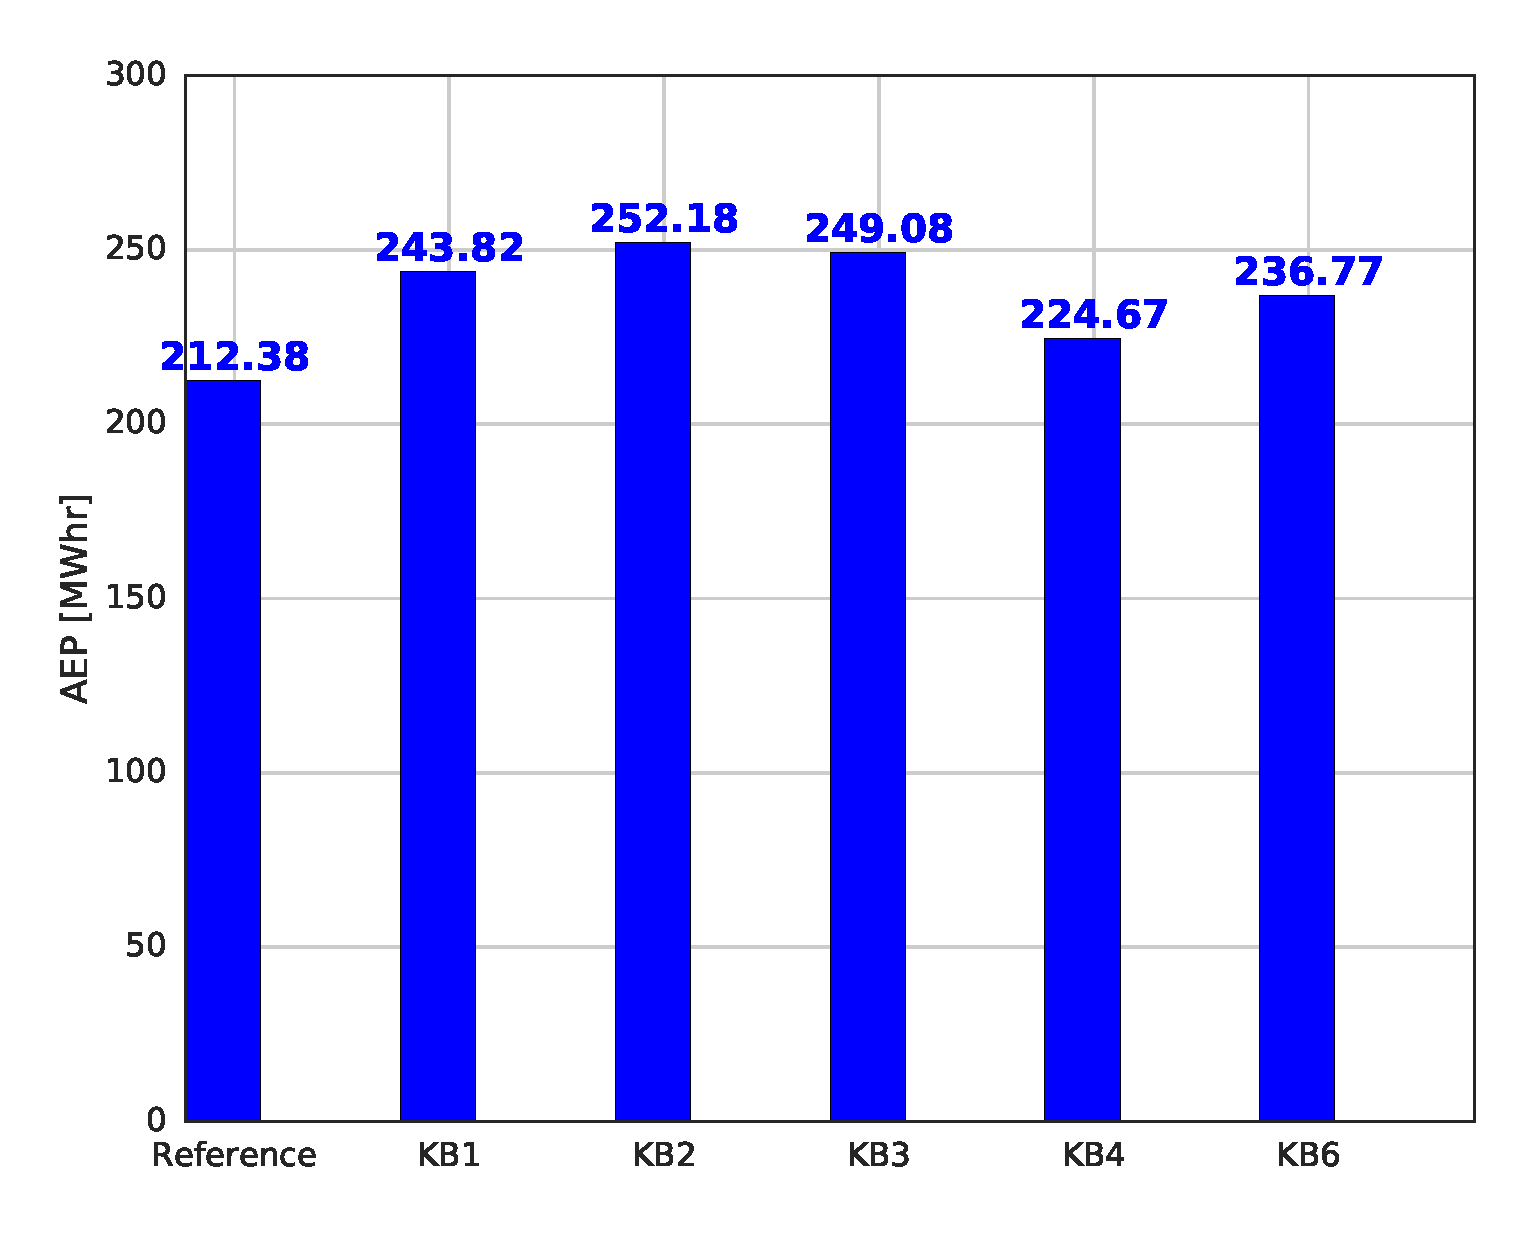
\includegraphics[width=.85\linewidth]{figures/KBcomp_AEPcomp.eps}
\end{center}
\caption{Annual energy production of the five optimized blades for a Weibull wind distribution with scale factor A=6.0 m/s and shape factor k= 2.0 [-].}
\label{fig:KB_AEP}
\end{figure}

\begin{figure}[!ht]
\begin{center}
	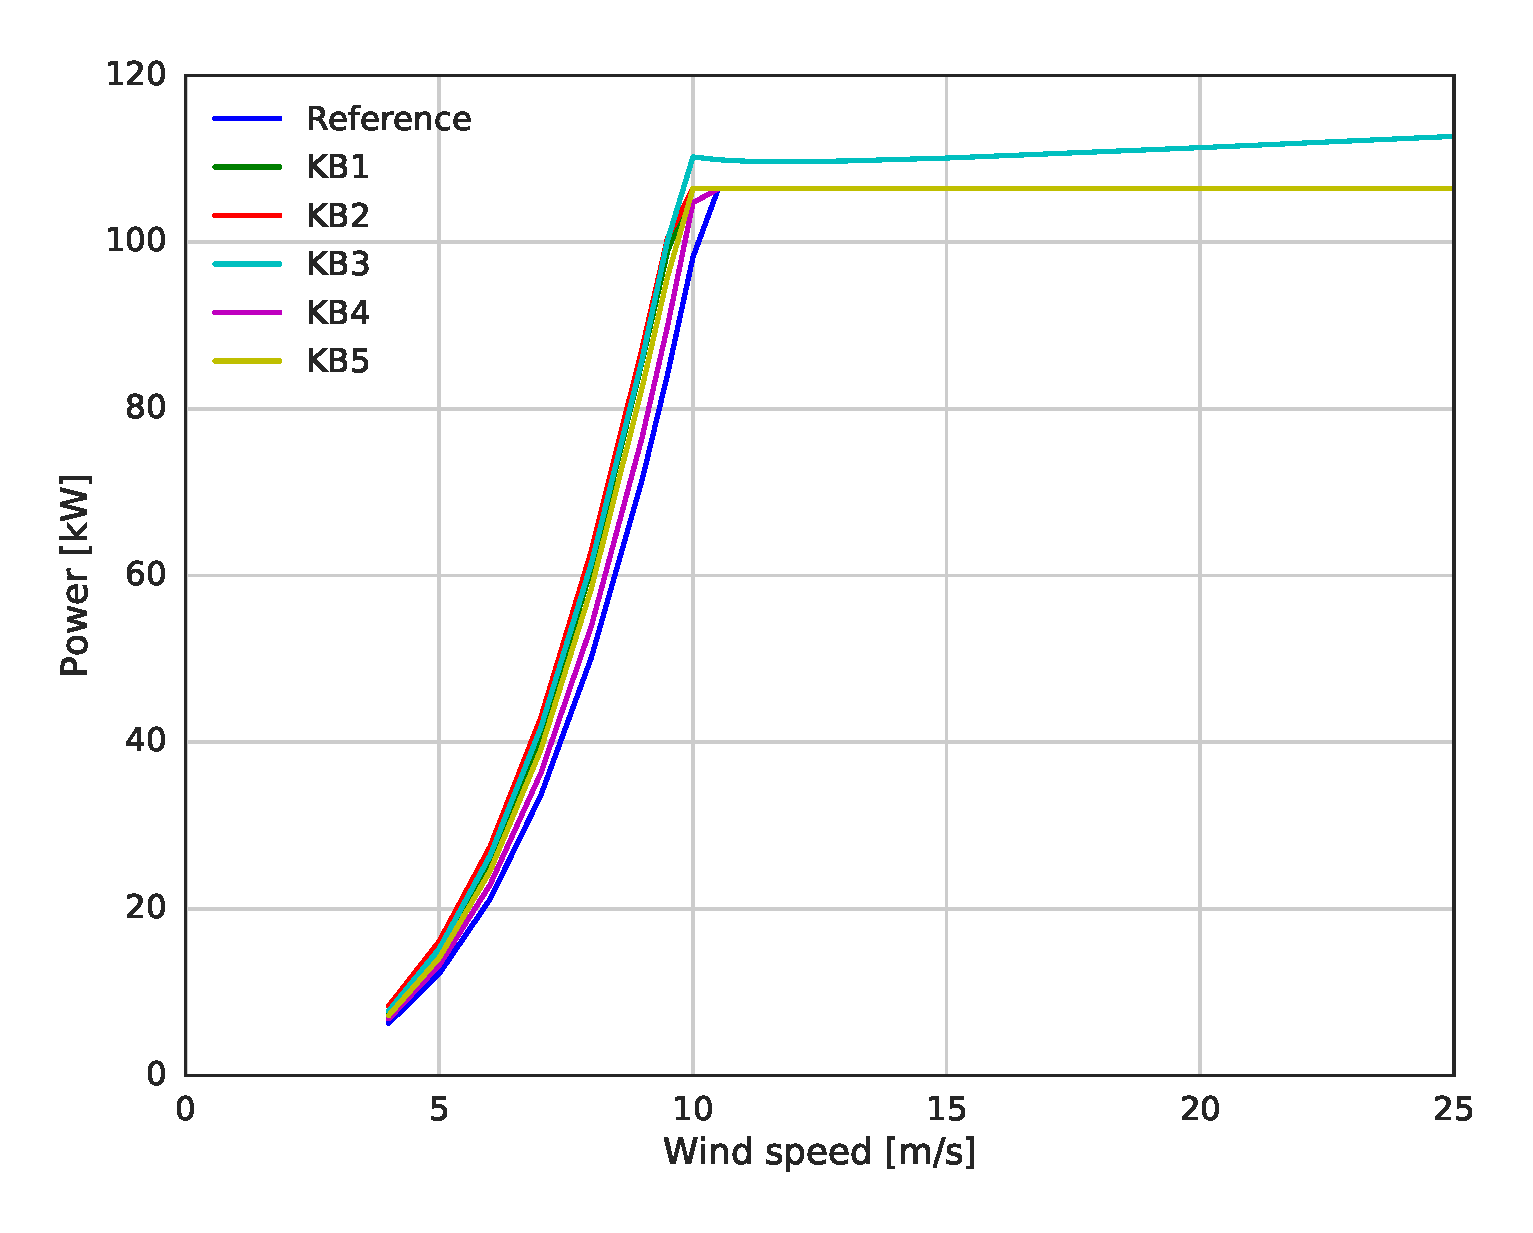
\includegraphics[width=.85\linewidth]{figures/KBcomp_power.eps}
\end{center}
\caption{Mechanical power as function of wind speed for the five optimized blades.}
\label{fig:power}
\end{figure}

%\begin{figure}[!ht]
%\begin{center}
%	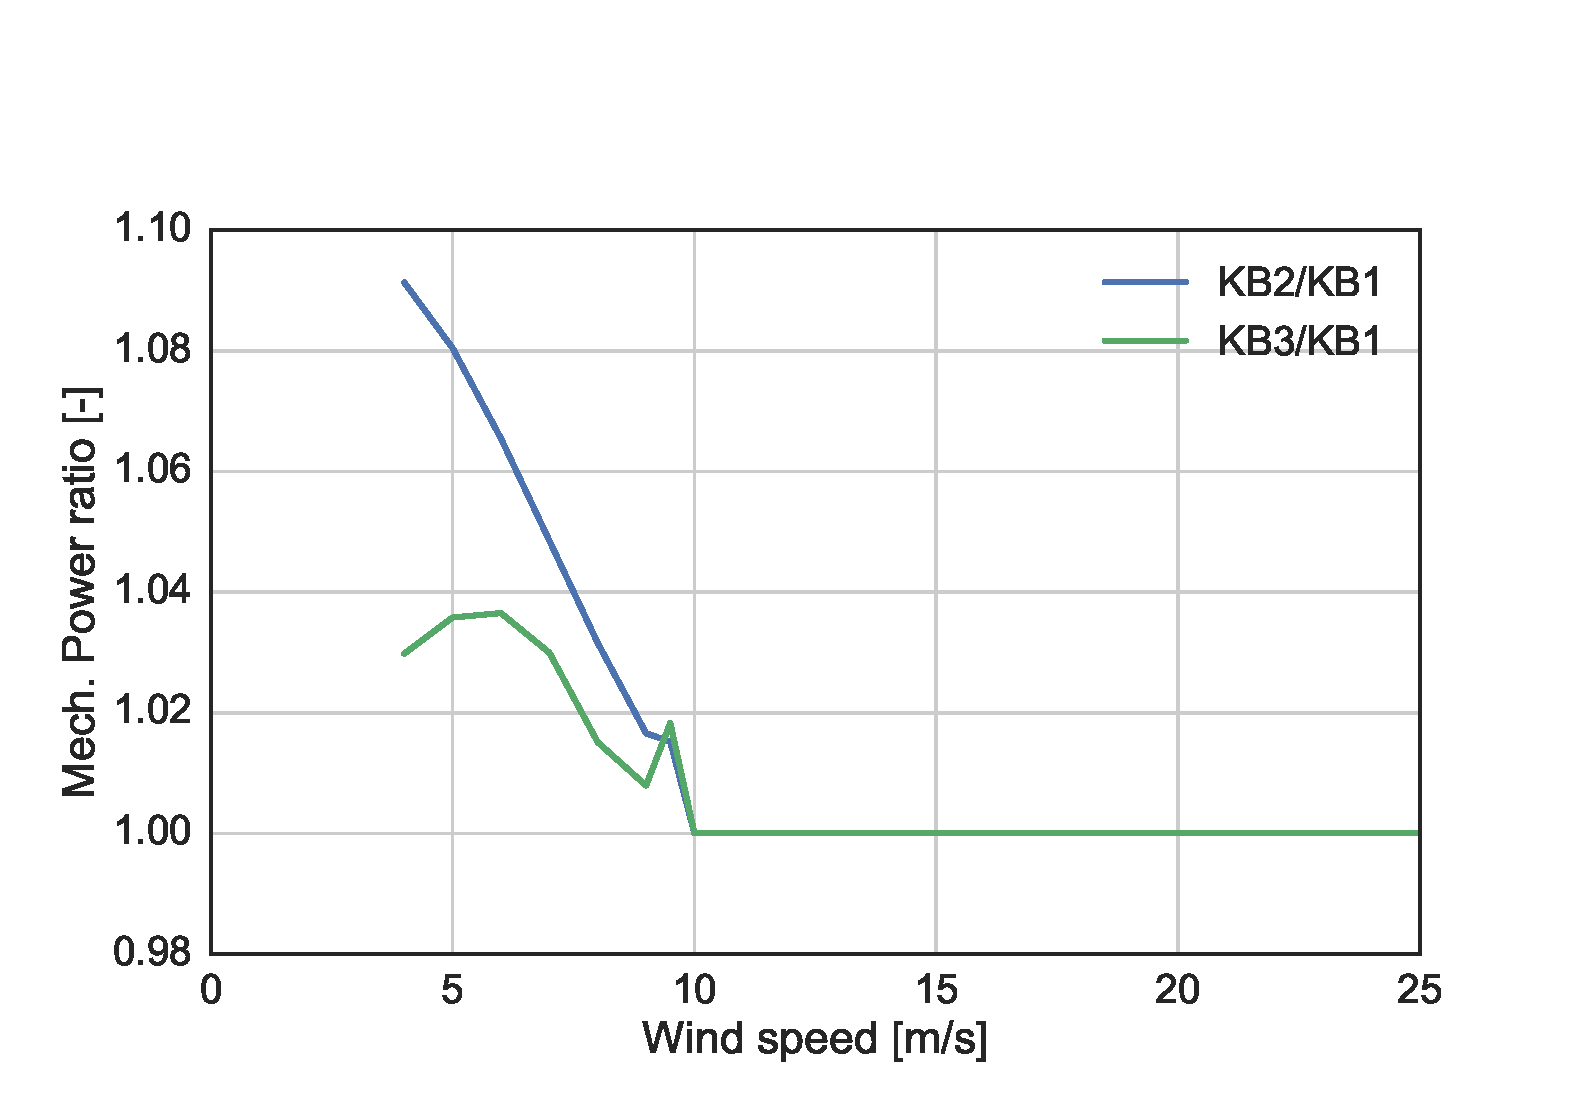
\includegraphics[width=.85\linewidth]{figures/KB_power_ratio.eps}
%\end{center}
%\caption{Ratio of mechanical power as function of wind speed for KB2 and KB3 relative to KB1.}
%\label{fig:powerratio}
%\end{figure}

\begin{figure}[!ht]
\begin{center}
	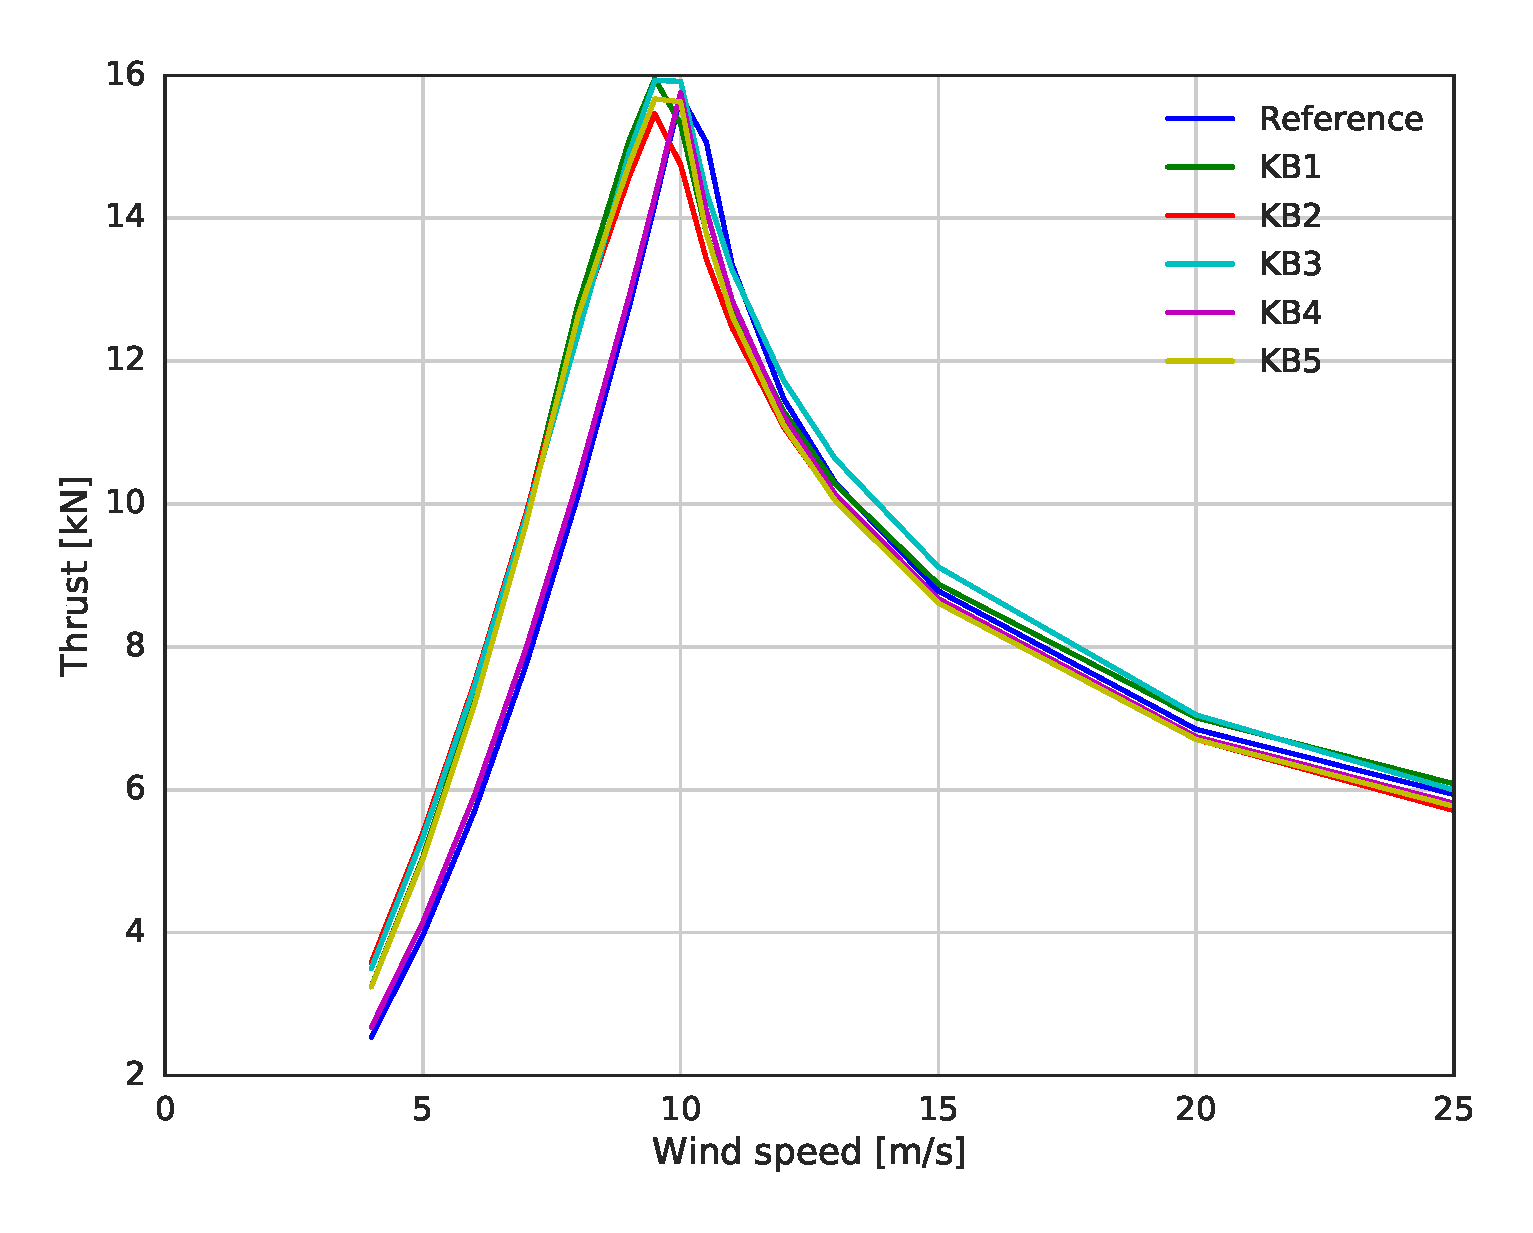
\includegraphics[width=.85\linewidth]{figures/KBcomp_thrust.eps}
\end{center}
\caption{Rotor thrust as function of wind speed for the five optimized blades.}
\label{fig:thrust}
\end{figure}

\begin{figure}[!ht]
\begin{center}
	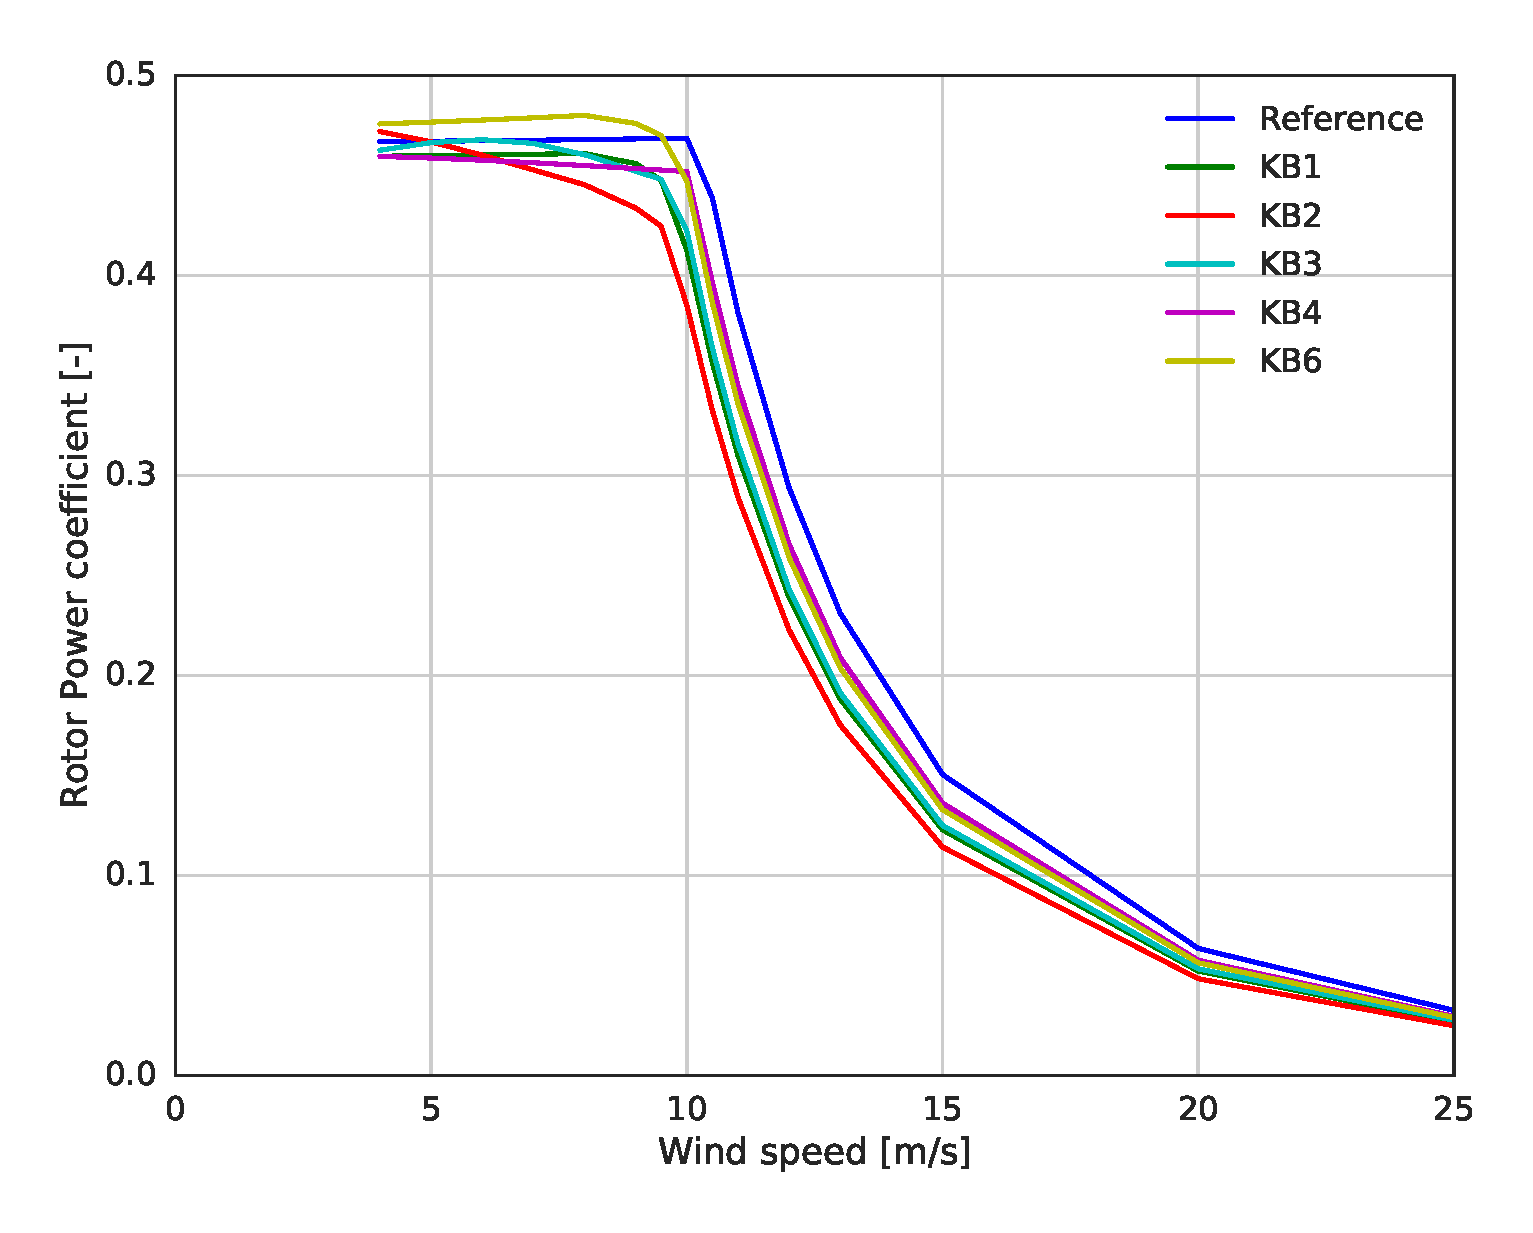
\includegraphics[width=.85\linewidth]{figures/KBcomp_Cp.eps}
\end{center}
\caption{Mechanical power coefficient as function of wind speed for the five optimized blades.}
\label{fig:cp}
\end{figure}

\begin{figure}[!ht]
\begin{center}
	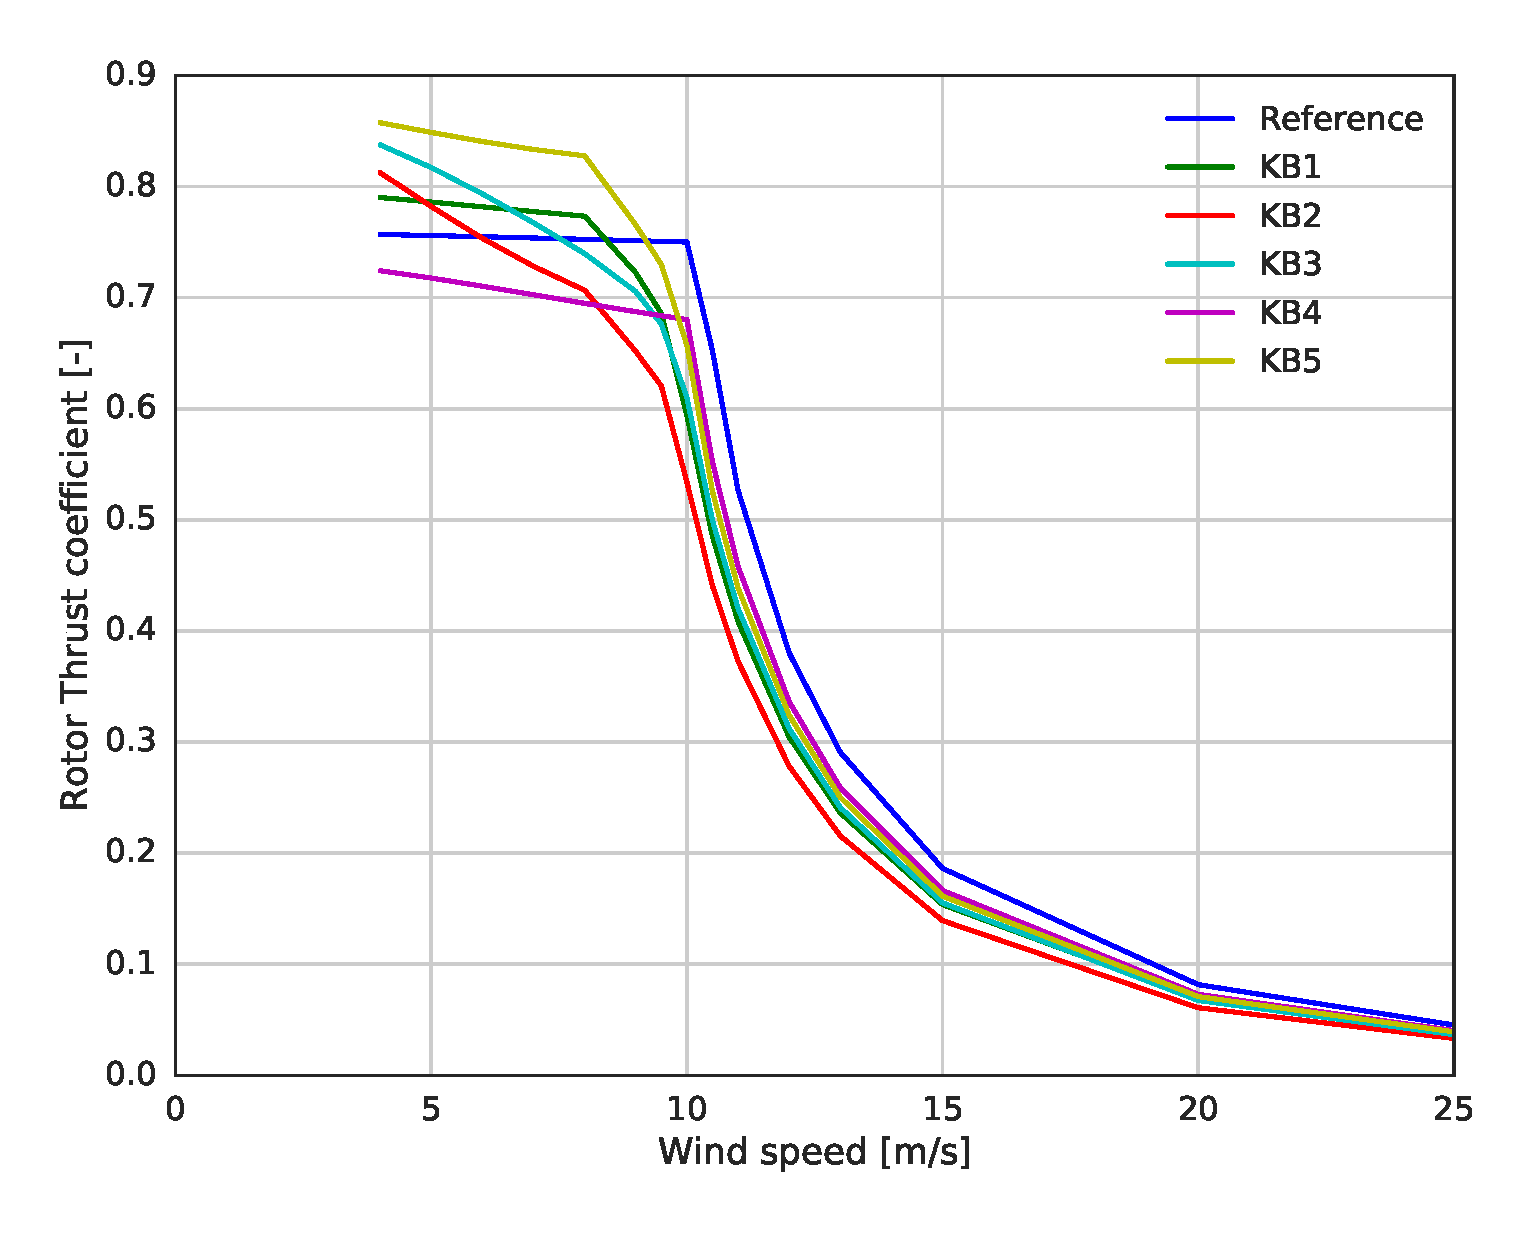
\includegraphics[width=.85\linewidth]{figures/KBcomp_CT.eps}
\end{center}
\caption{Rotor thrust coefficient as function of wind speed for the five optimized blades.}
\label{fig:ct}
\end{figure}

\begin{figure}[!ht]
\begin{center}
	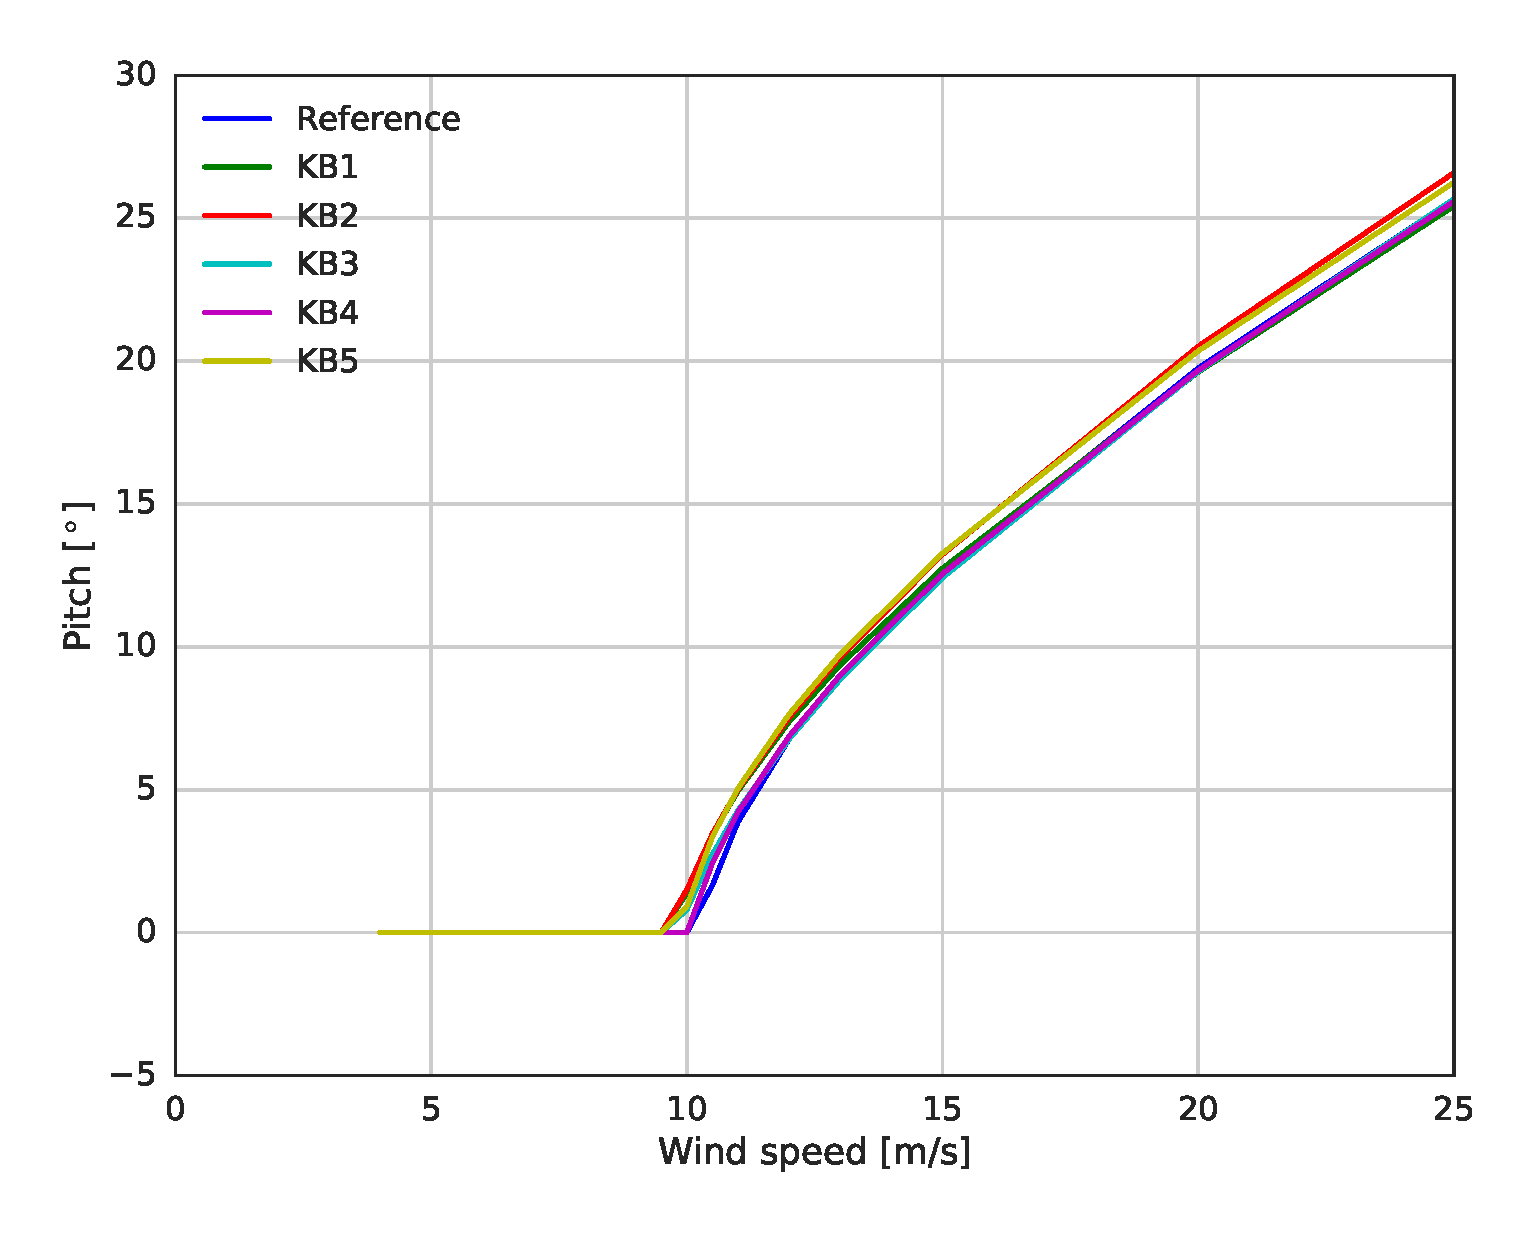
\includegraphics[width=.85\linewidth]{figures/KBcomp_pitch.eps}
\end{center}
\caption{Blade pitch as function of wind speed for the five optimized blades.}
\label{fig:pitch}
\end{figure}

\begin{figure}[!ht]
\begin{center}
	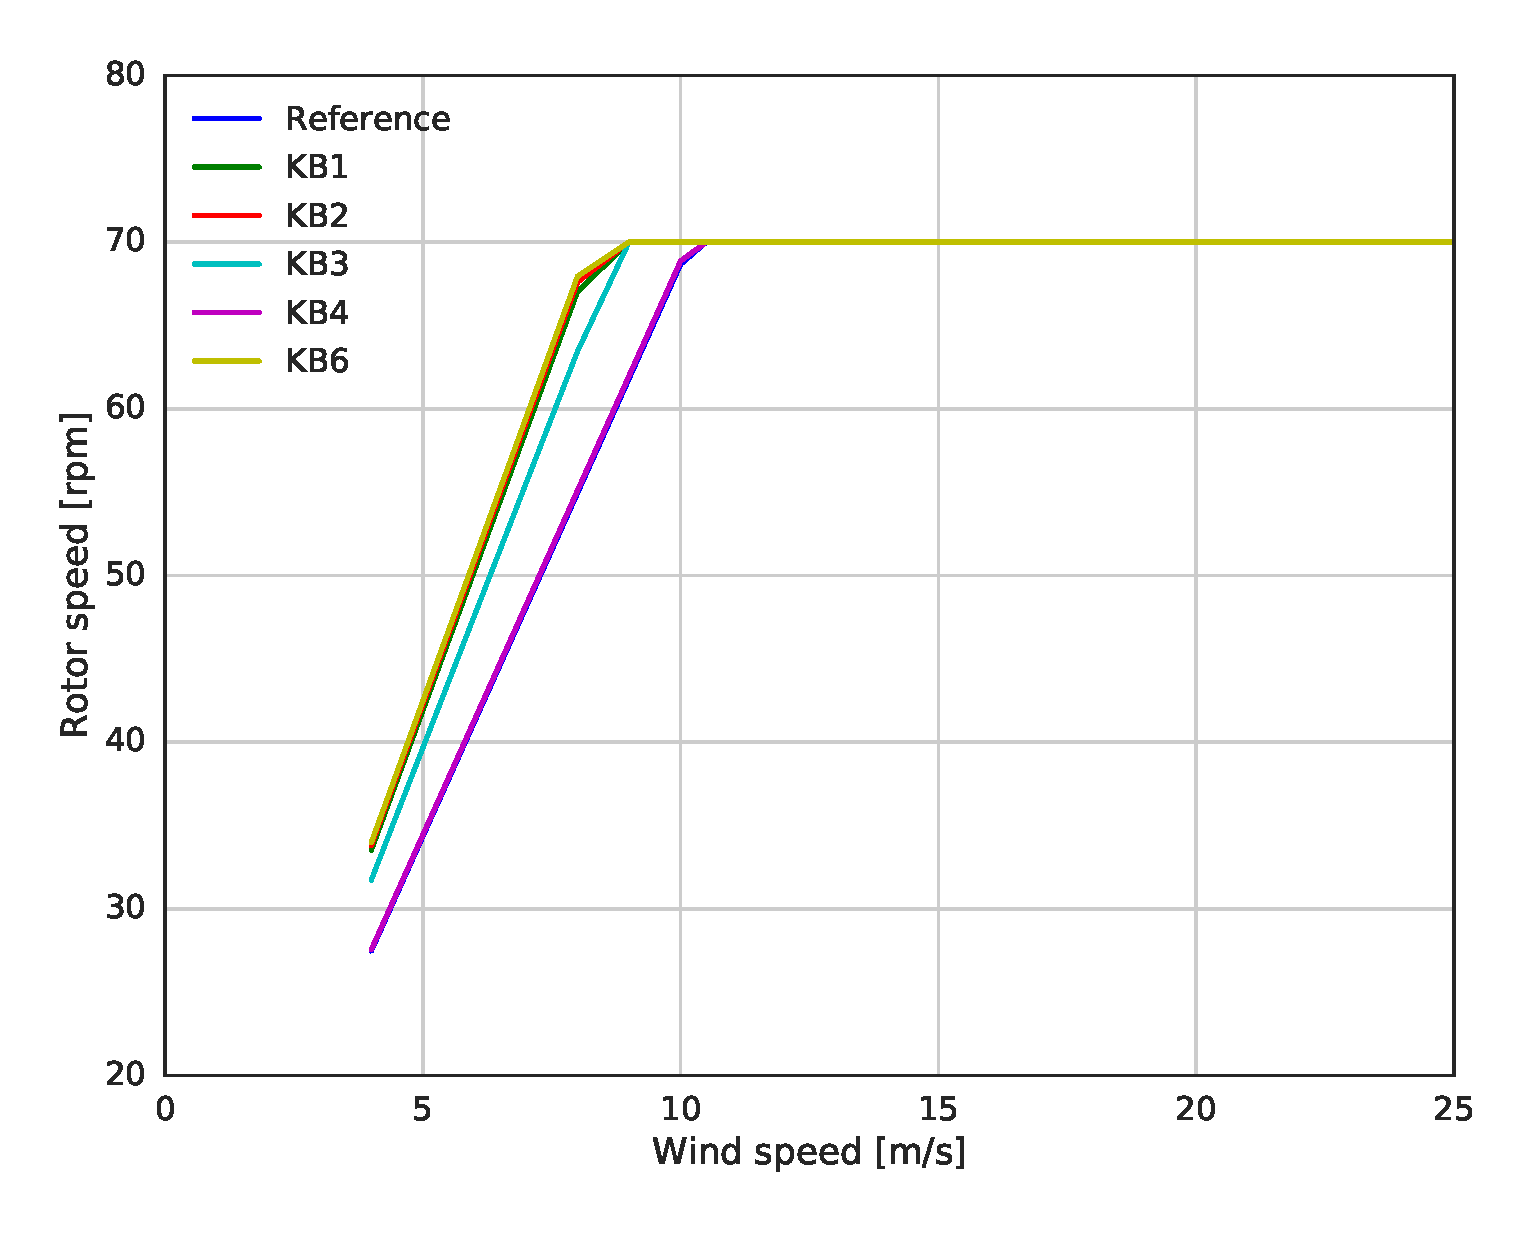
\includegraphics[width=.85\linewidth]{figures/KBcomp_rpm.eps}
\end{center}
\caption{Rotor speed as function of wind speed for the five optimized blades.}
\label{fig:rpm}
\end{figure}

\clearpage

Figures \ref{fig:chord} to \ref{fig:prebend} show the blade planform for the three blades compared to the reference.
All three blades have a more slender planform than the reference resulting from the high TSR, which enables driving down blade mass.
Both KB2 and KB3 have different twist distributions towards the blade tip due to the torsional coupling.
The optimized blades generally have higher airfoil relative thicknesses, particularly near mid-span, where there are the highest demands for stiffness and strength.
Towards the root the relative thicknesses decrease due to the high chord which provides sufficient blade thickness and therefore stiffness.
The optimizer can also alter the position of the cross-section relative to the blade axis, referred to as pitch axis aft leading edge.
This affects the positioning of the spar cap within the cross-section as well as the aerodynamic pitch moment.
For all blades, the cross-section is moved forward towards the tip, somewhat less pronounced for the KB3 blade. 

\begin{figure}[!ht]
\begin{center}
	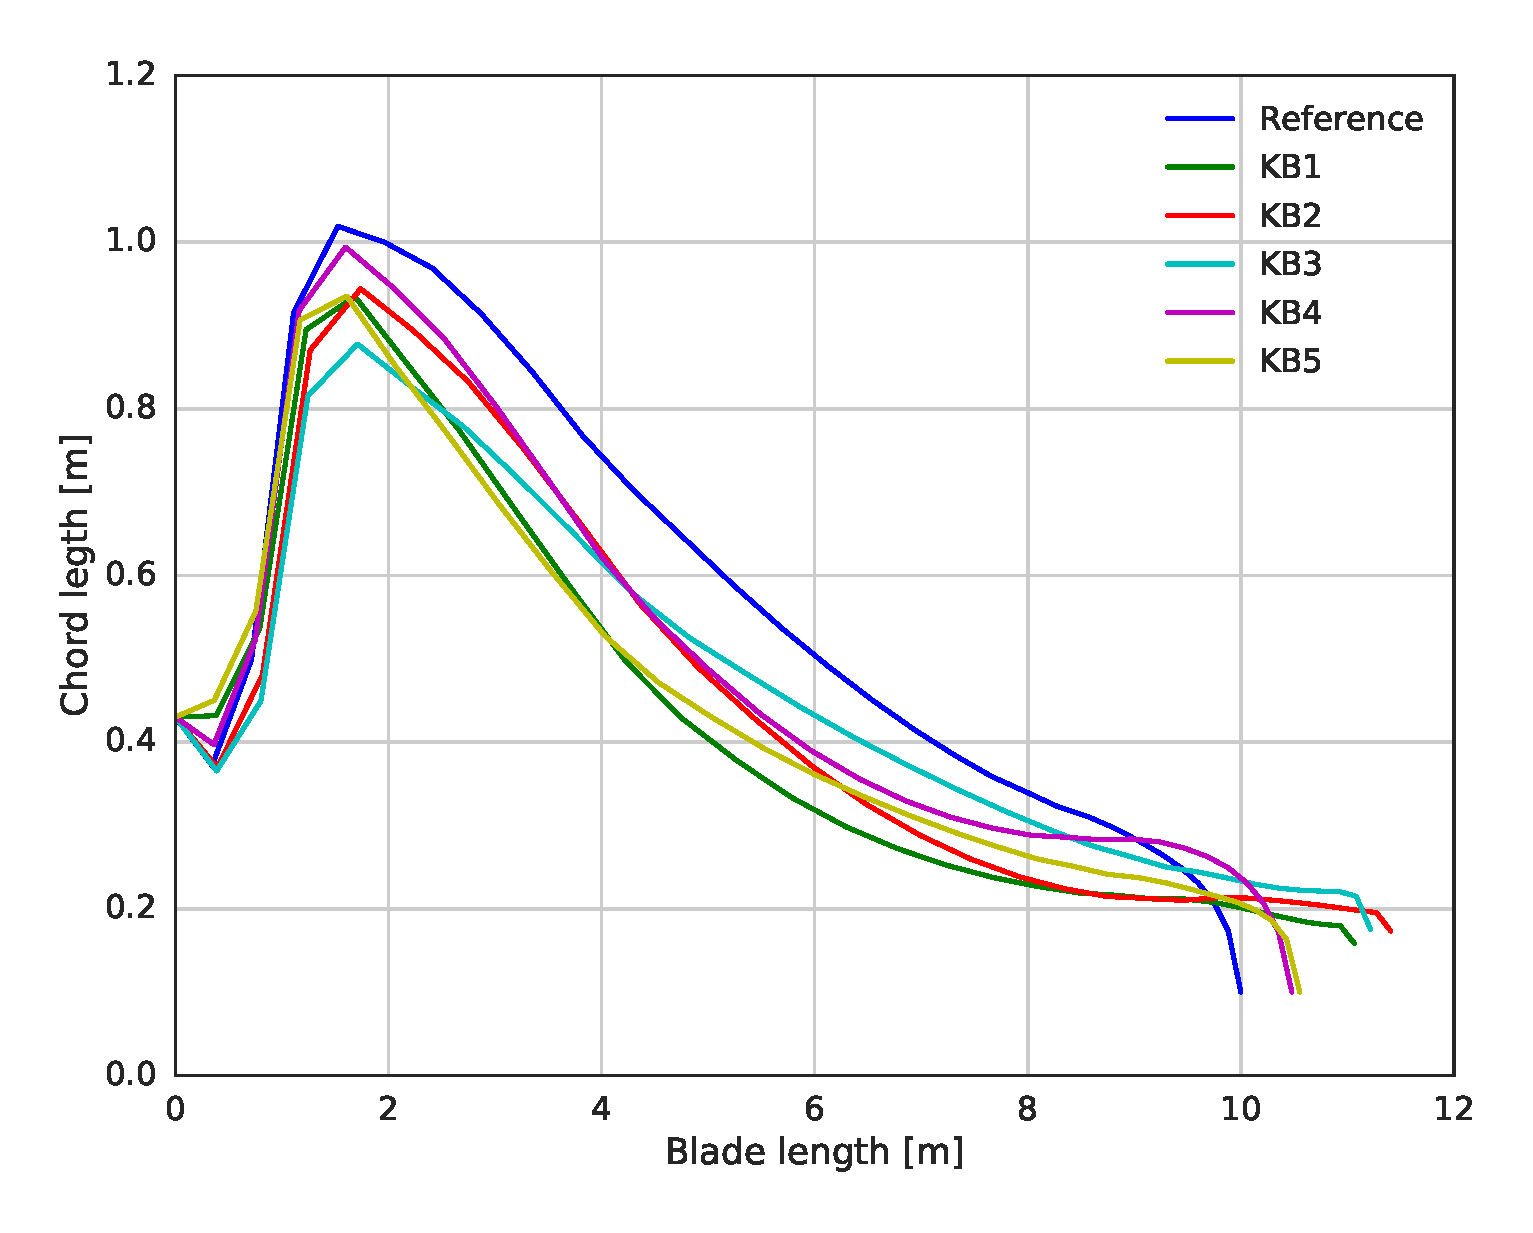
\includegraphics[width=.85\linewidth]{figures/KBcomp_chord.eps}
\end{center}
\caption{Blade chord distributions for the five optimized blades.}
\label{fig:chord}
\end{figure}


\begin{figure}[!ht]
\begin{center}
	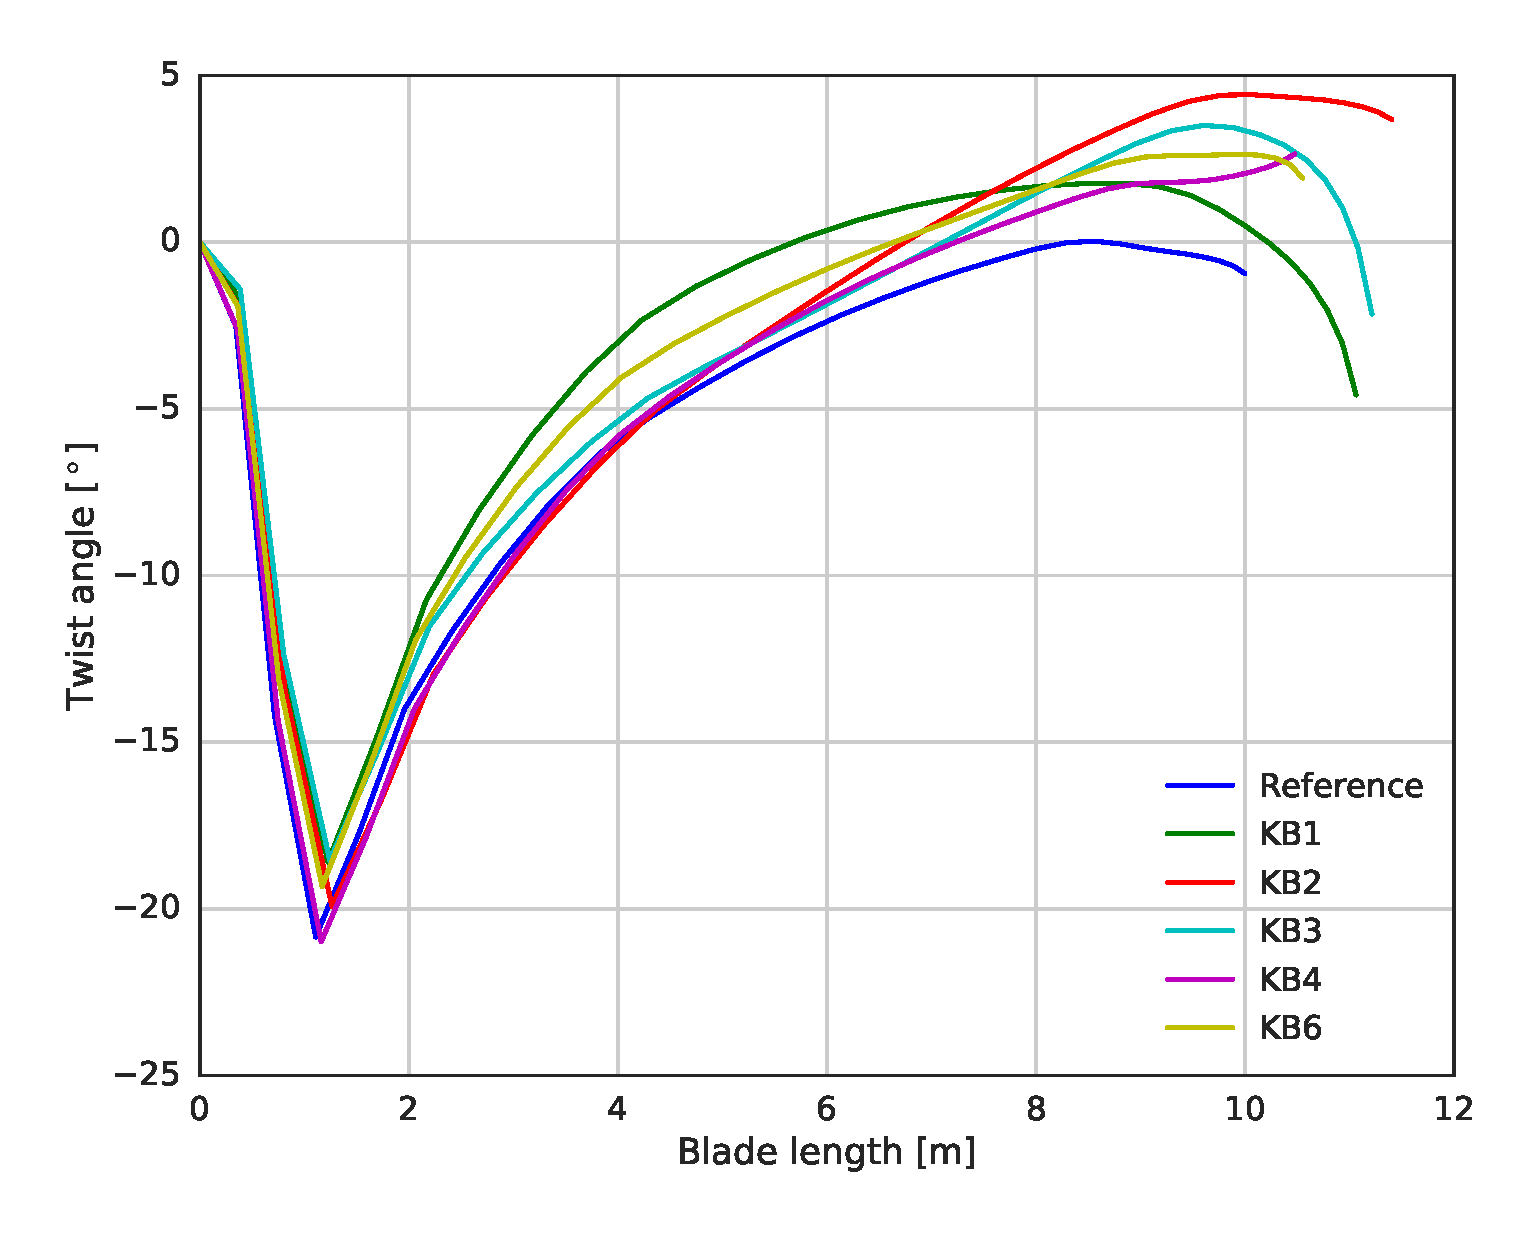
\includegraphics[width=.85\linewidth]{figures/KBcomp_twist.eps}
\end{center}
\caption{Blade twist distributions for the five optimized blades.}
\label{fig:twist}
\end{figure}

\begin{figure}[!ht]
\begin{center}
	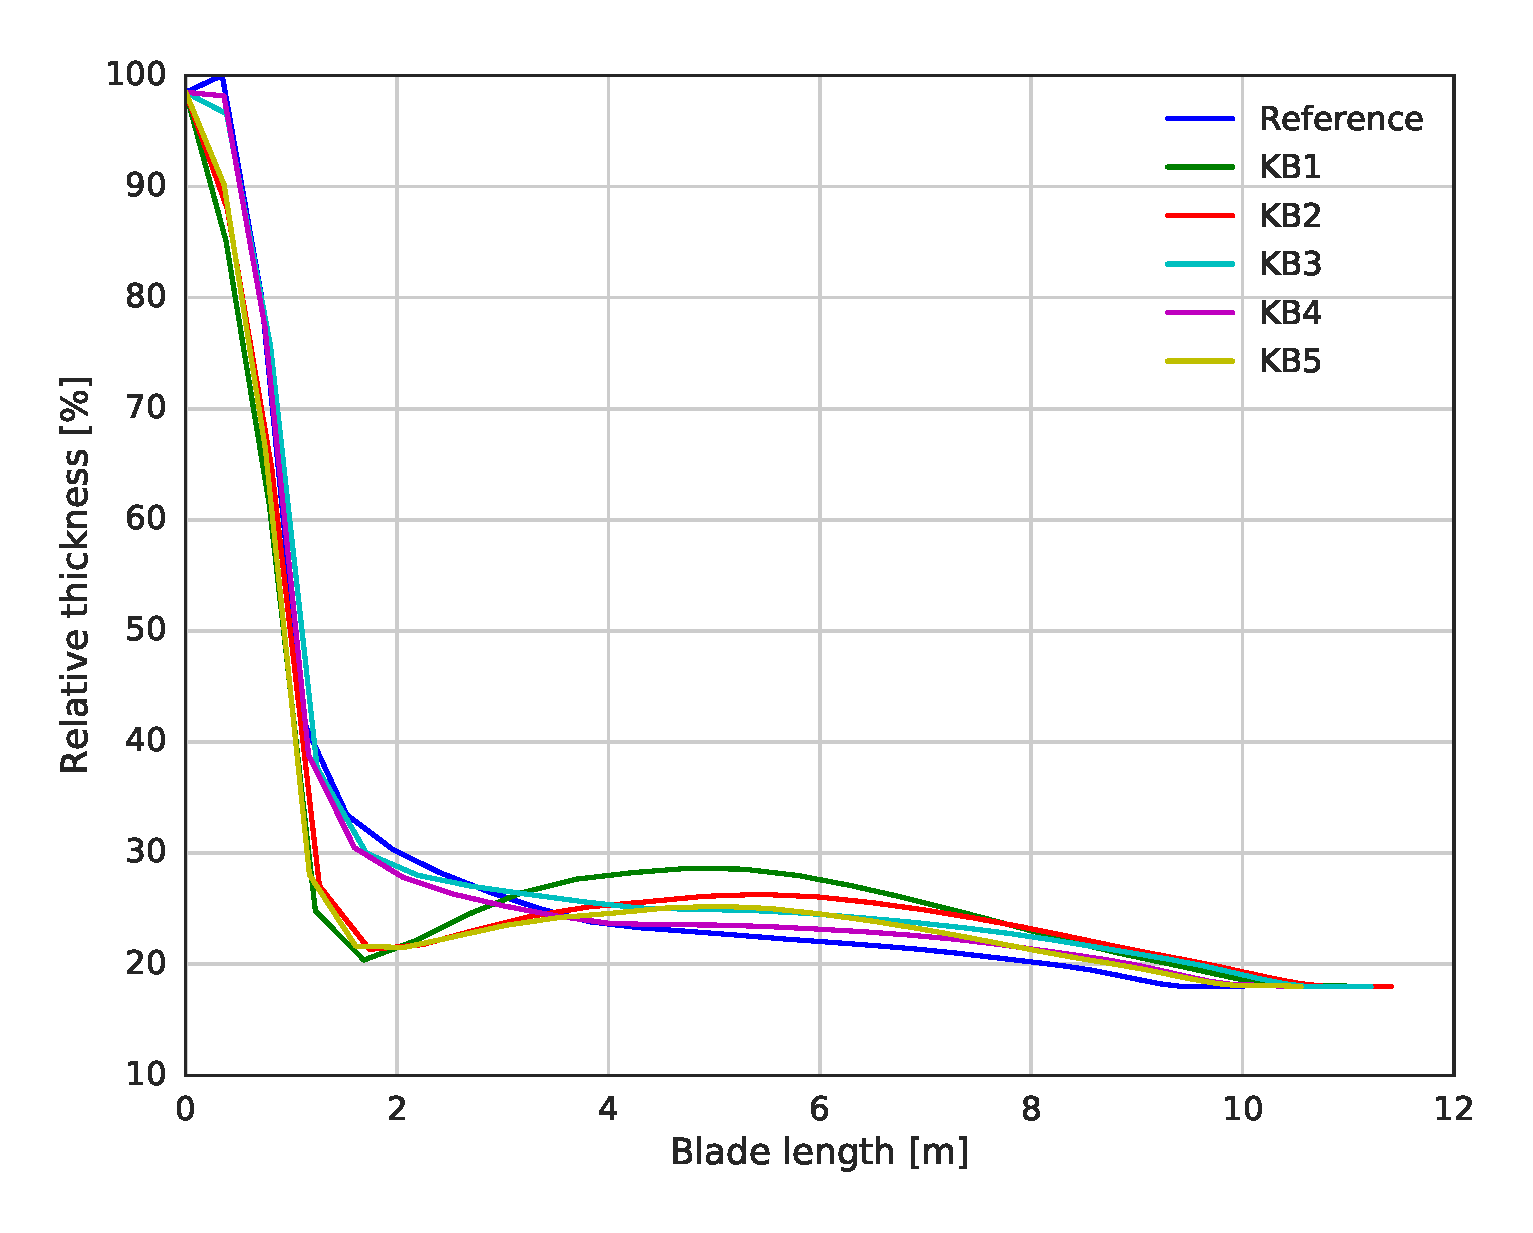
\includegraphics[width=.85\linewidth]{figures/KBcomp_rthick.eps}
\end{center}
\caption{Blade relative thickness distributions for the five optimized blades.}
\label{fig:rthick}
\end{figure}


\begin{figure}[!ht]
\begin{center}
	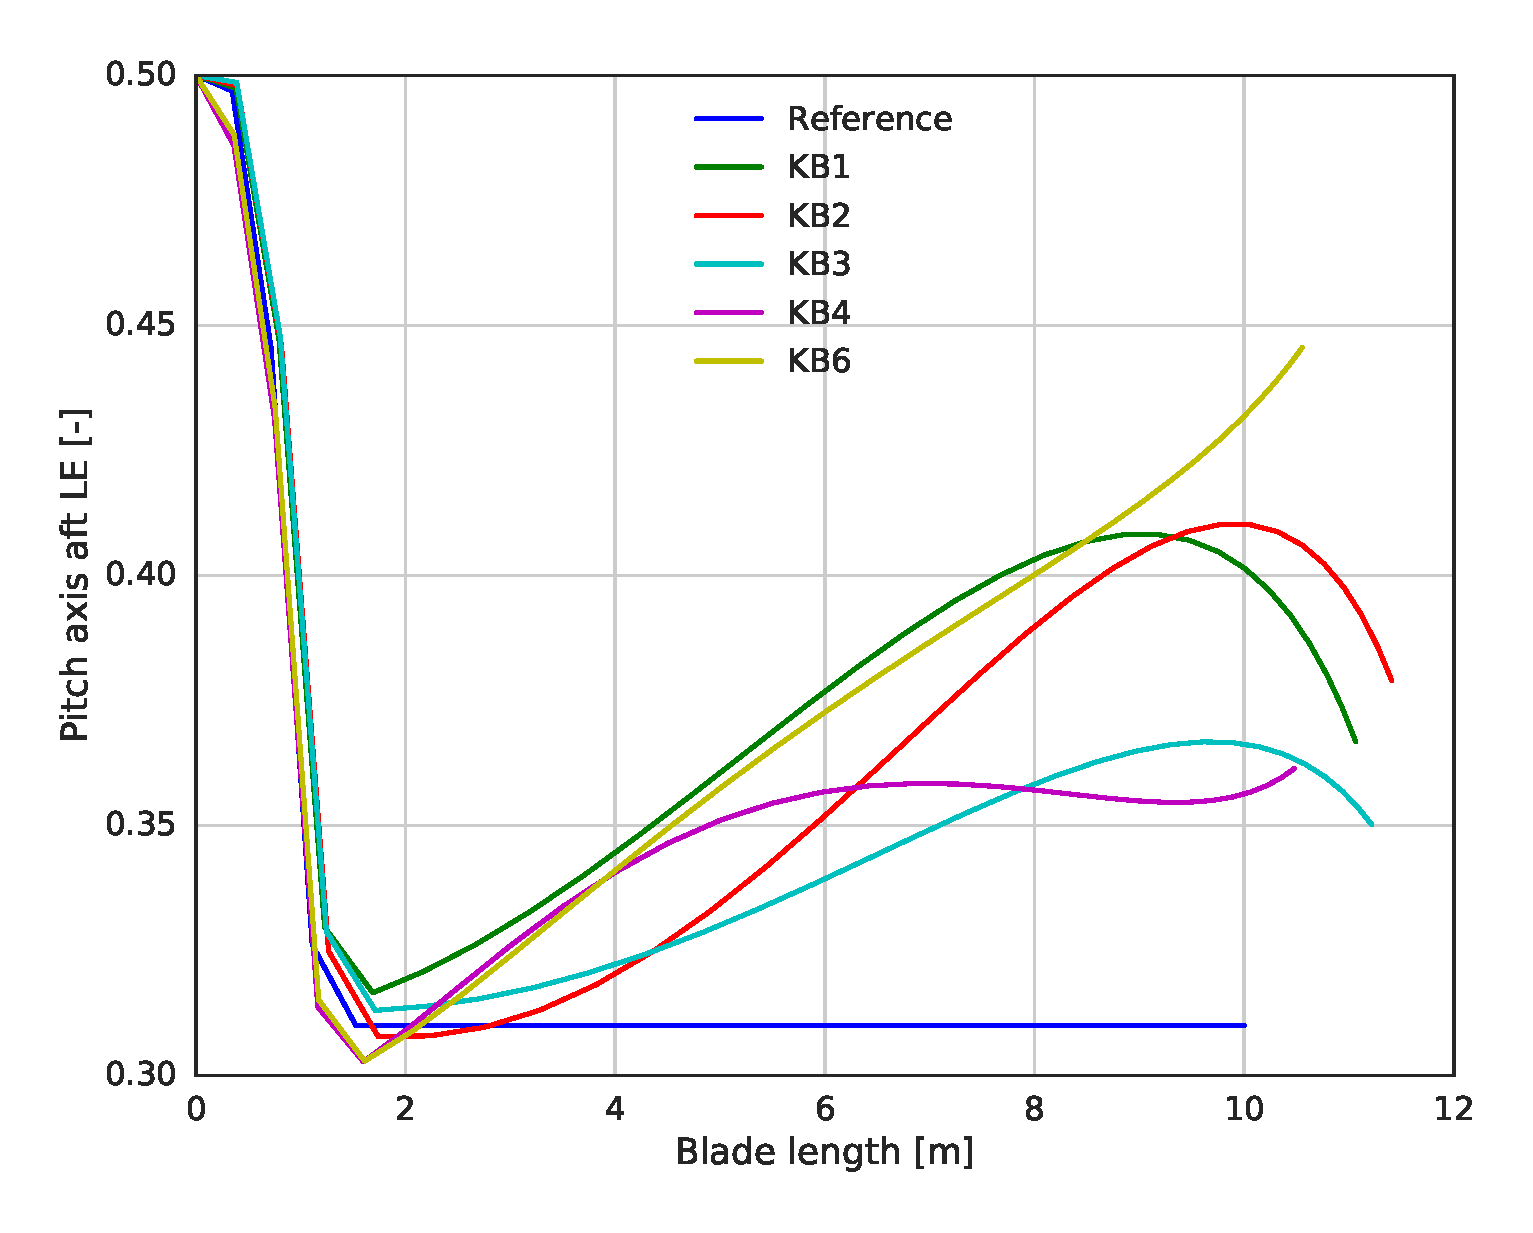
\includegraphics[width=.85\linewidth]{figures/KBcomp_ple.eps}
\end{center}
\caption{Non-dimensionalized blade axis leading edge offset distributions for the five optimized blades.}
\label{fig:p_le}
\end{figure}

\begin{figure}[!ht]
\begin{center}
	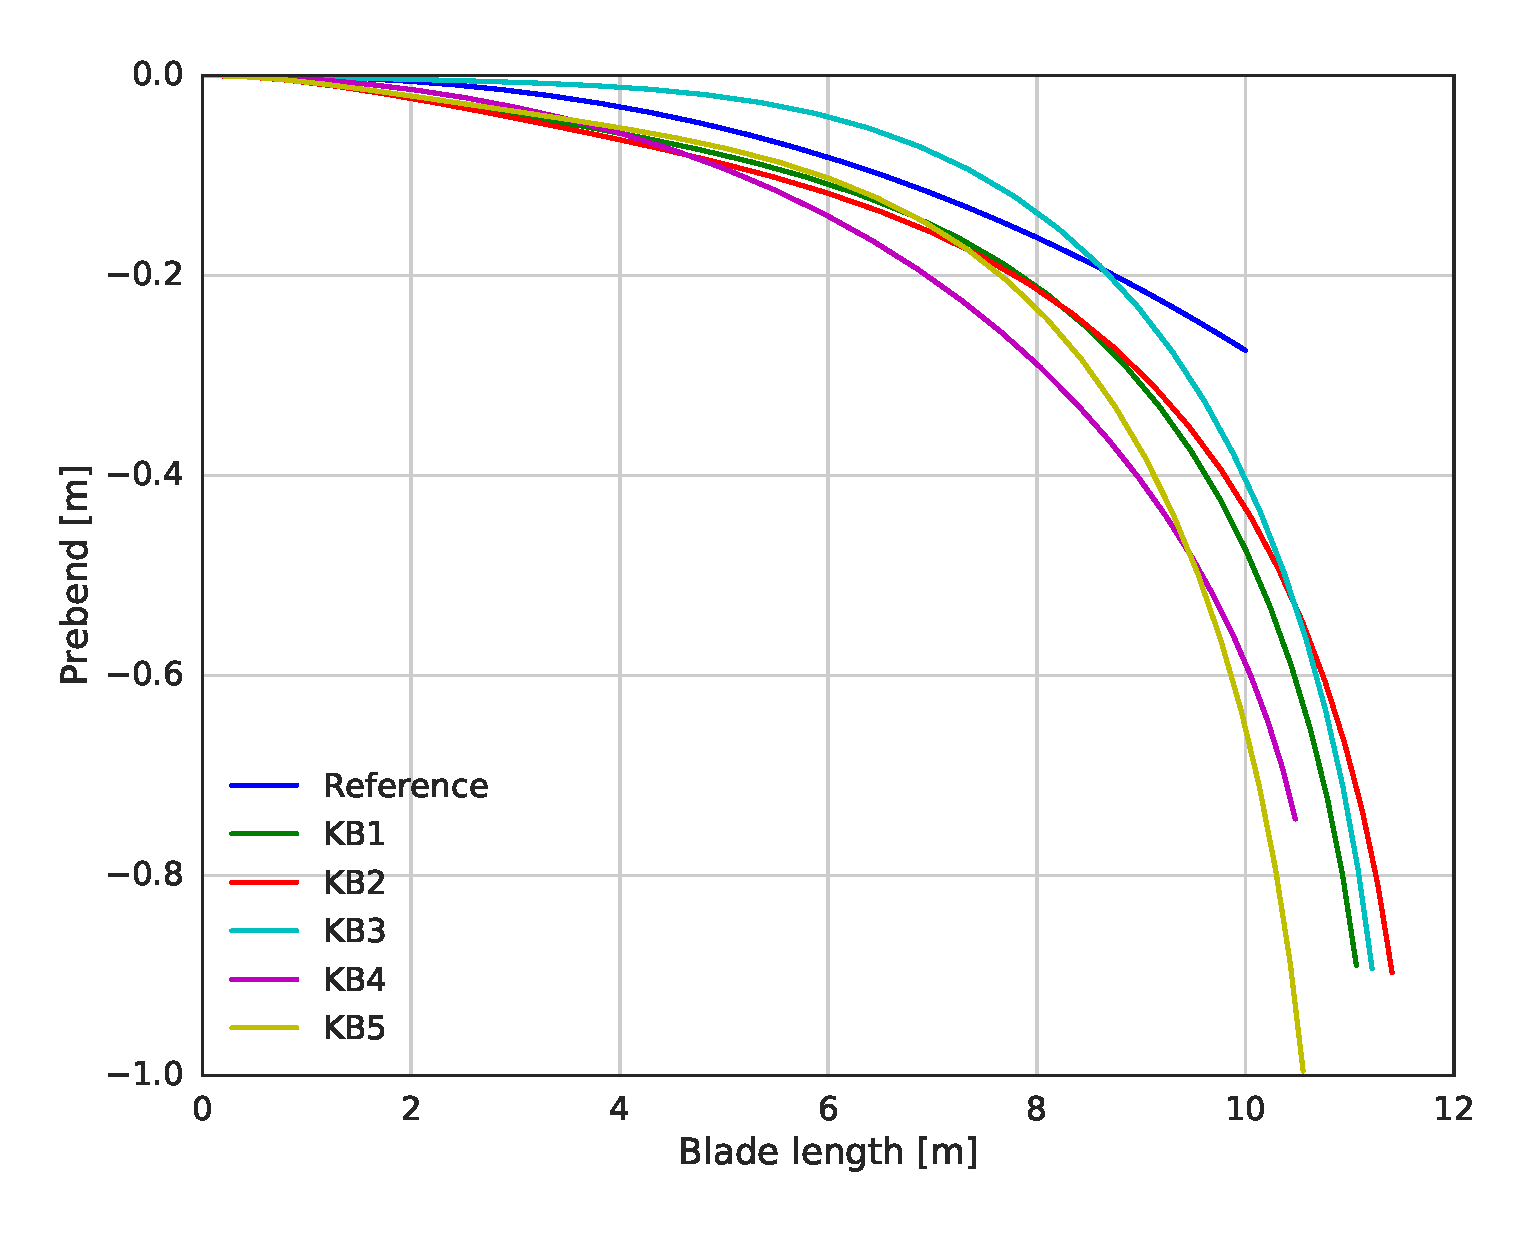
\includegraphics[width=.85\linewidth]{figures/KBcomp_prebend.eps}
\end{center}
\caption{Blade pre-bend distributions for the five optimized blades.}
\label{fig:prebend}
\end{figure}

\begin{figure}[!ht]
\begin{center}
	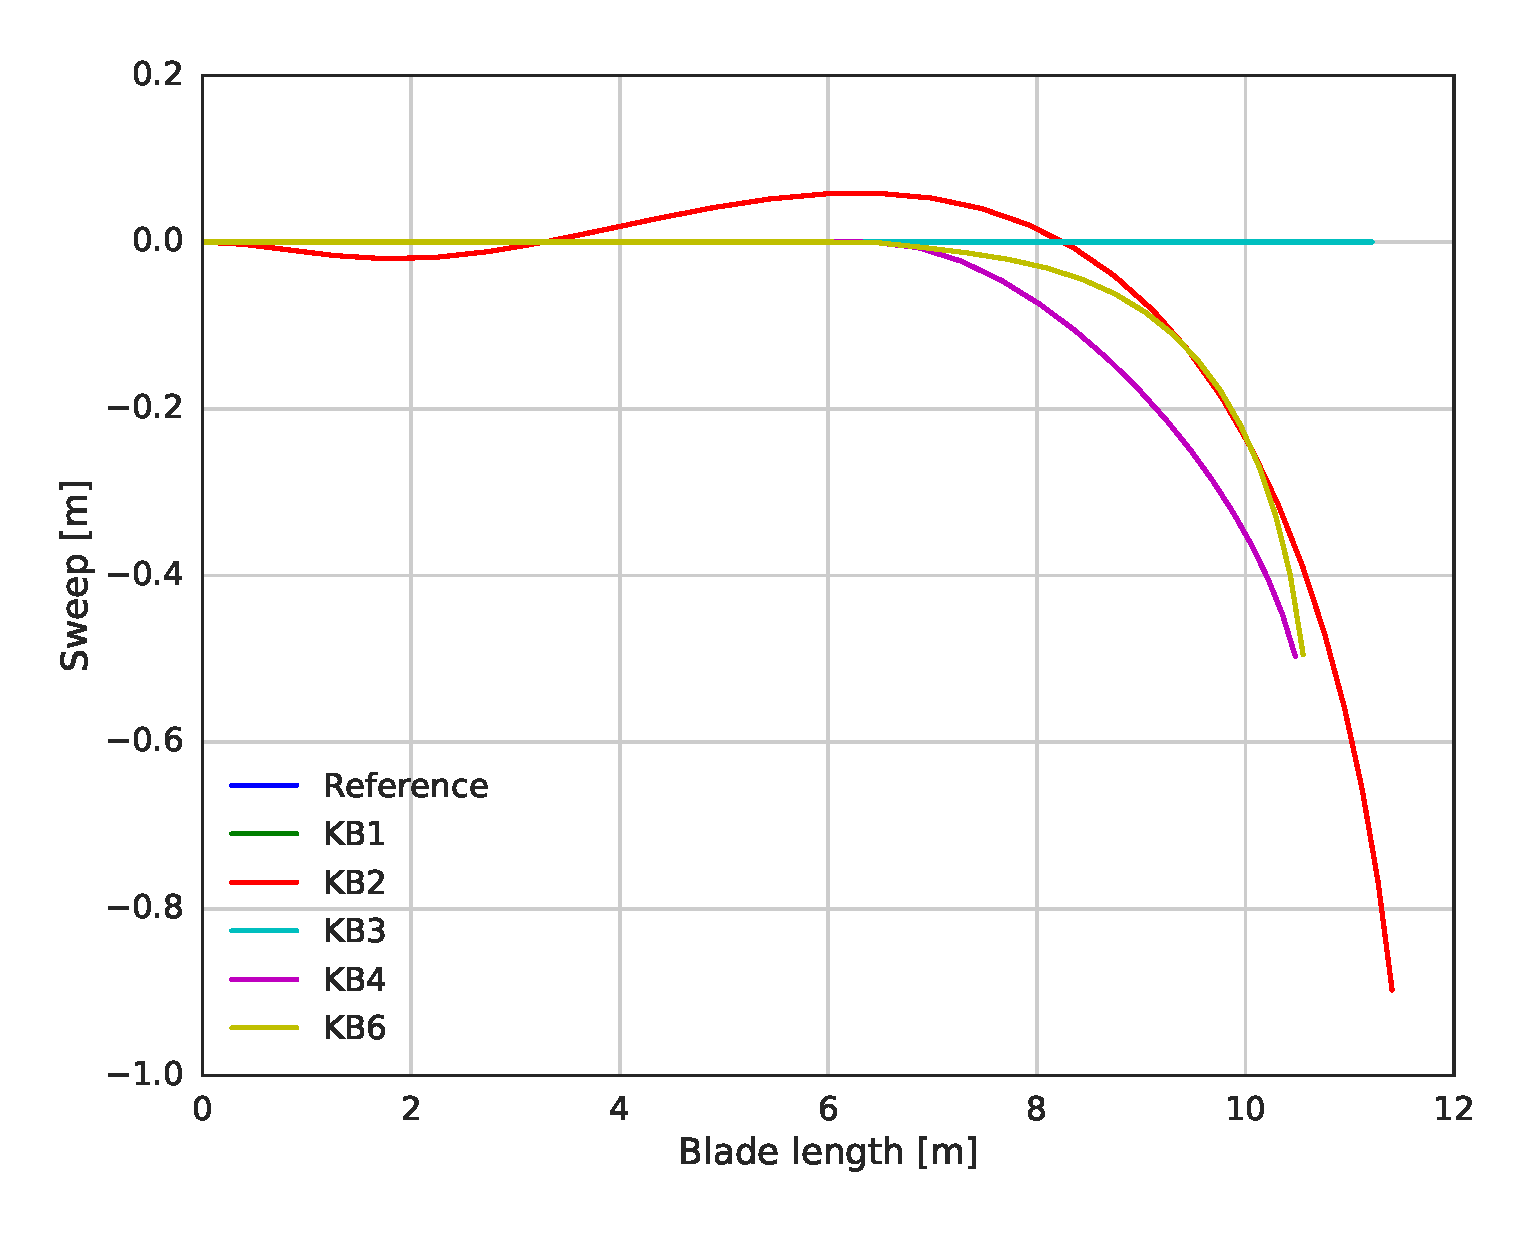
\includegraphics[width=.85\linewidth]{figures/KBcomp_sweep.eps}
\end{center}
\caption{Blade sweep distributions for the five optimized blades.}
\label{fig:sweep}
\end{figure}

\subsection{Structural Design}

The overall structural topology is the same for all three blades, shown in Figure \ref{fig:loftedstructure_baseline_tipview}.
As summarized in the optimization setup, Table \ref{tab:dv_summary}, the spar cap width was allowed to change linearly from root to tip.
Changing cap width did, however, not change the distance between the two main shear webs, see Figure \ref{fig:cross_section_def} for a schematic of the cross-section parametrization.

Figure \ref{fig:capwidth} shows the resulting spar cap widths for the three blade designs compared to the Reference design.
The two blades without sweep, KB1 and KB3, result in an increased cap width in the blade root, whereas the swept design ends up with a more slender spar cap.  

\begin{figure}[!ht]
\begin{center}
	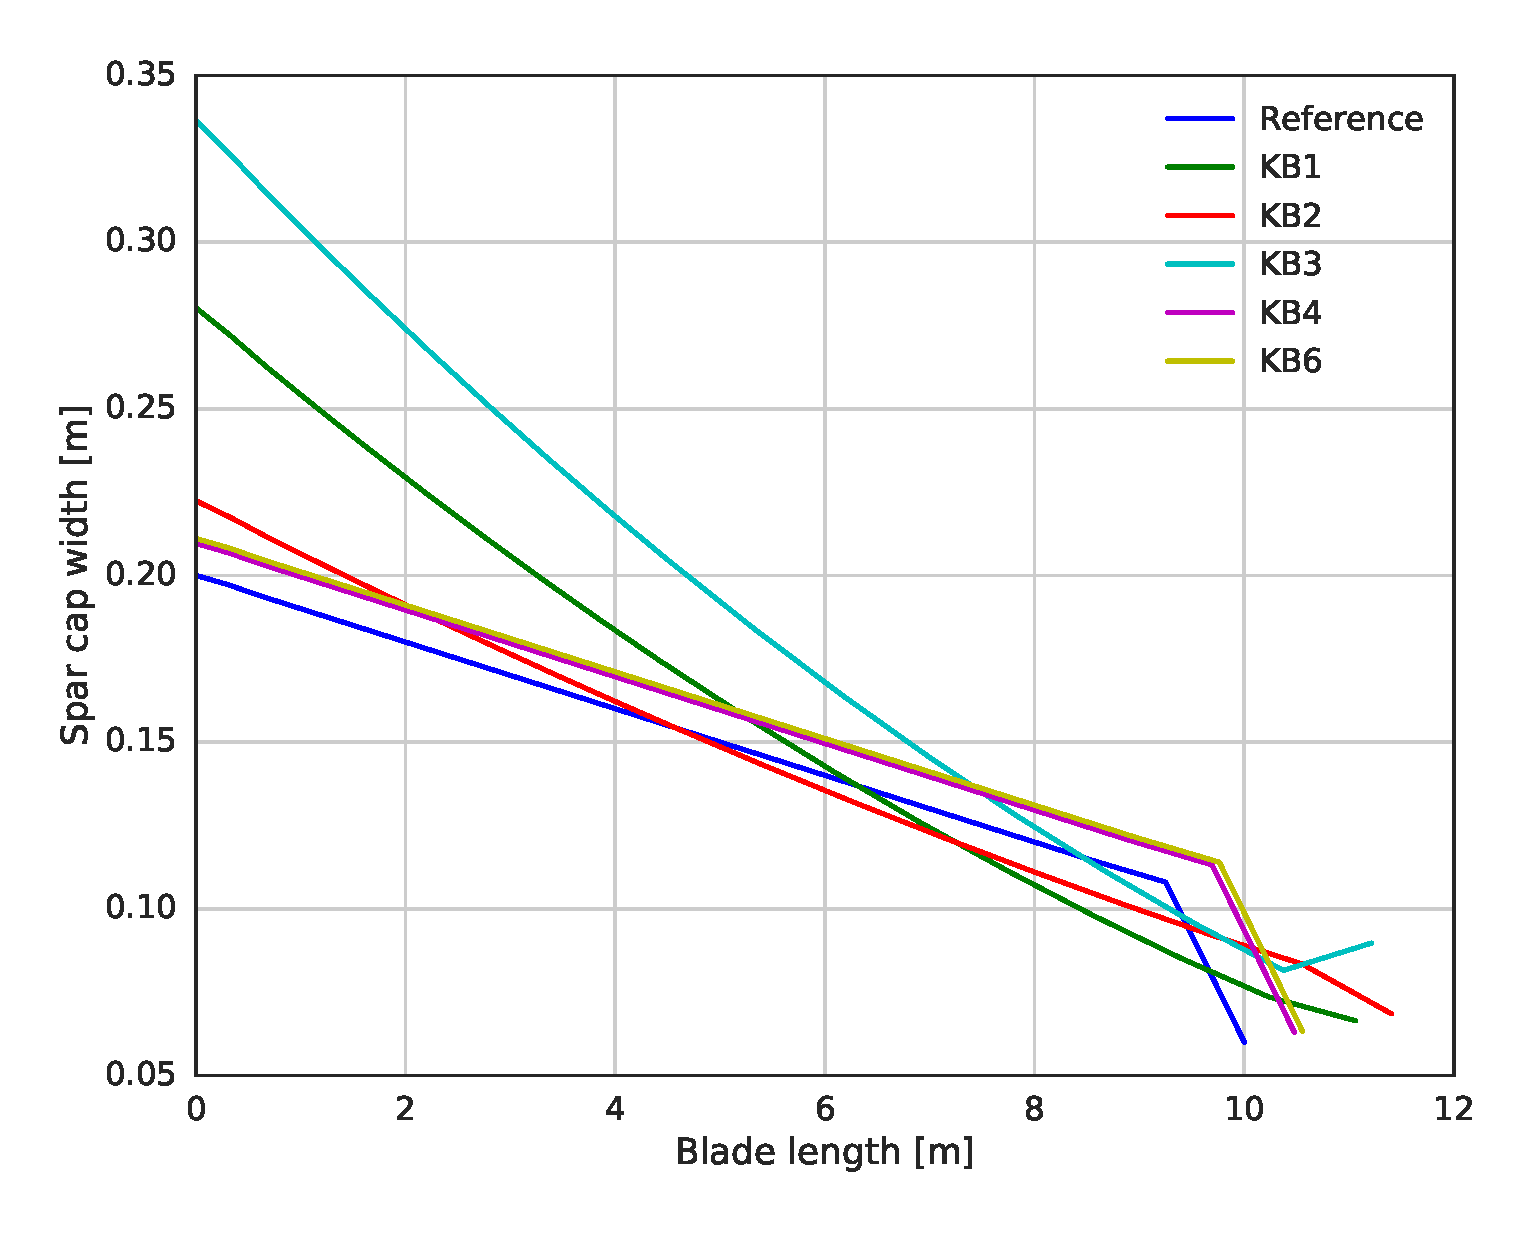
\includegraphics[width=.85\linewidth]{figures/KBcomp_spar_cap_width.eps}
\end{center}
\caption{Blade spar cap width distributions for the five optimized blades.}
\label{fig:capwidth}
\end{figure}

Figures \ref{fig:tipview} and \ref{fig:topview} show the lofted blade shape seen from the tip and top indicating the locations of region division points, spar cap, and shear webs.

\begin{figure}[!ht]
\begin{center}
	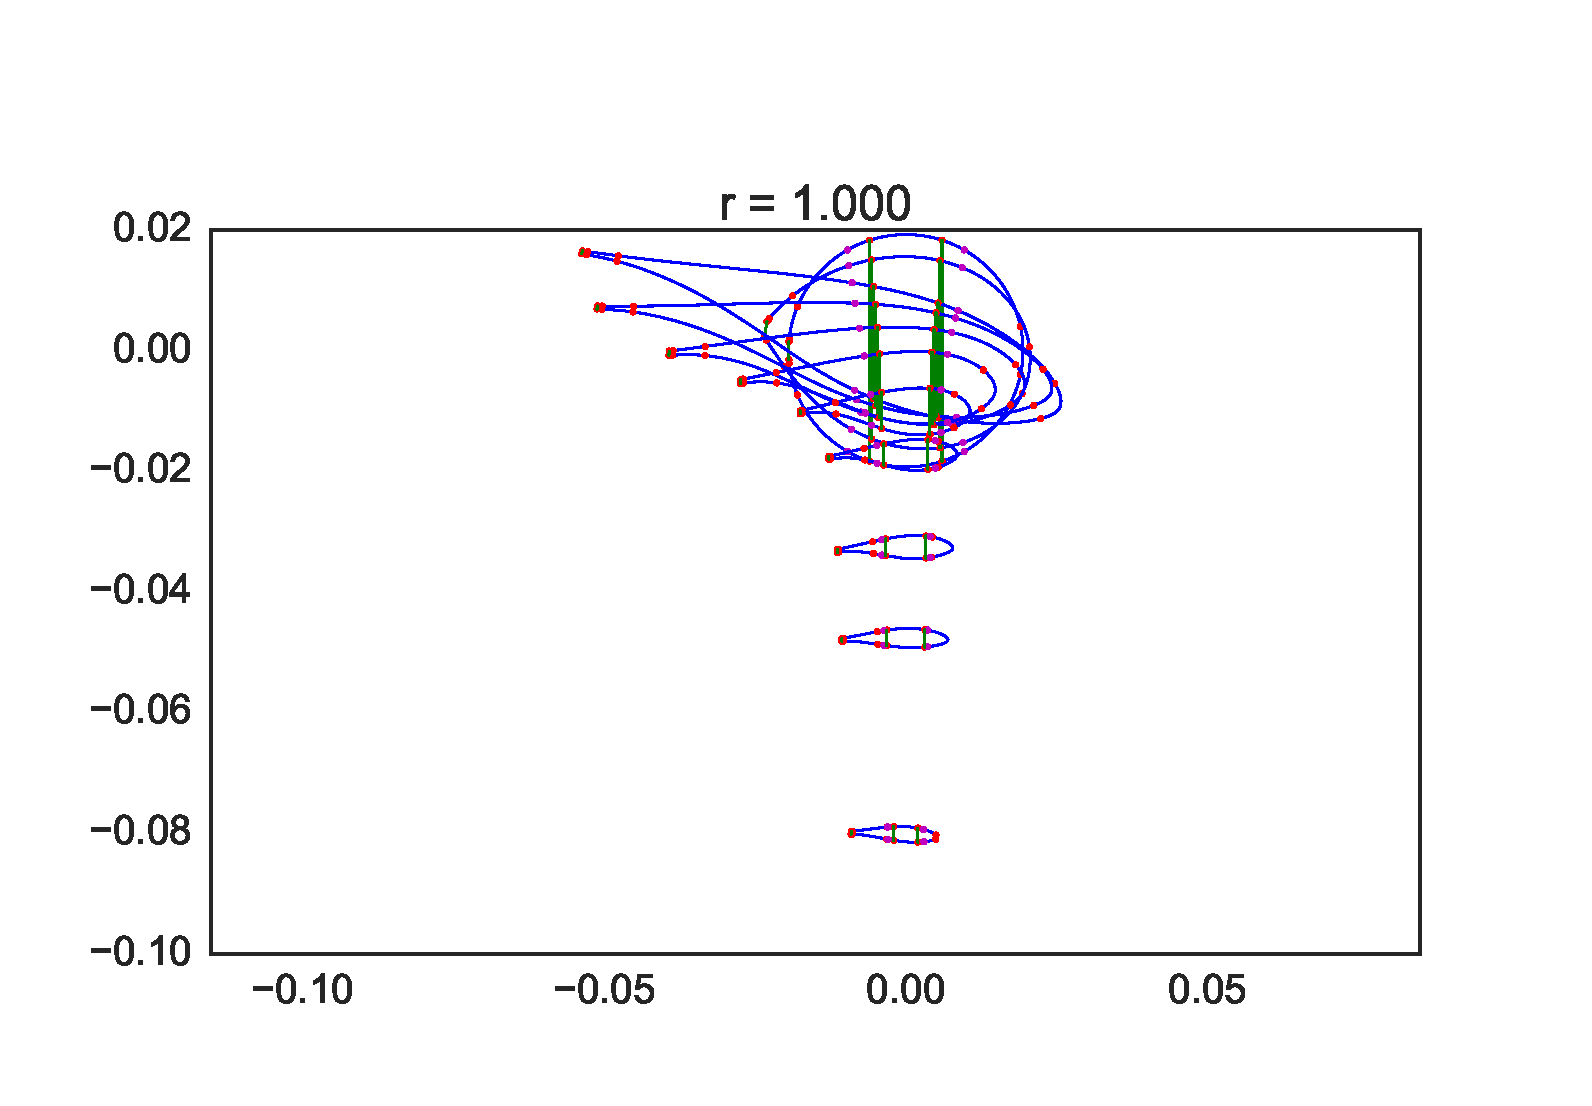
\includegraphics[width=.85\linewidth]{figures/KB1_tipview.eps}
\end{center}
\caption{Tipview schematic of the KB1 blade structure.}
\label{fig:tipview}
\end{figure}

\begin{figure}[!ht]
\begin{center}
	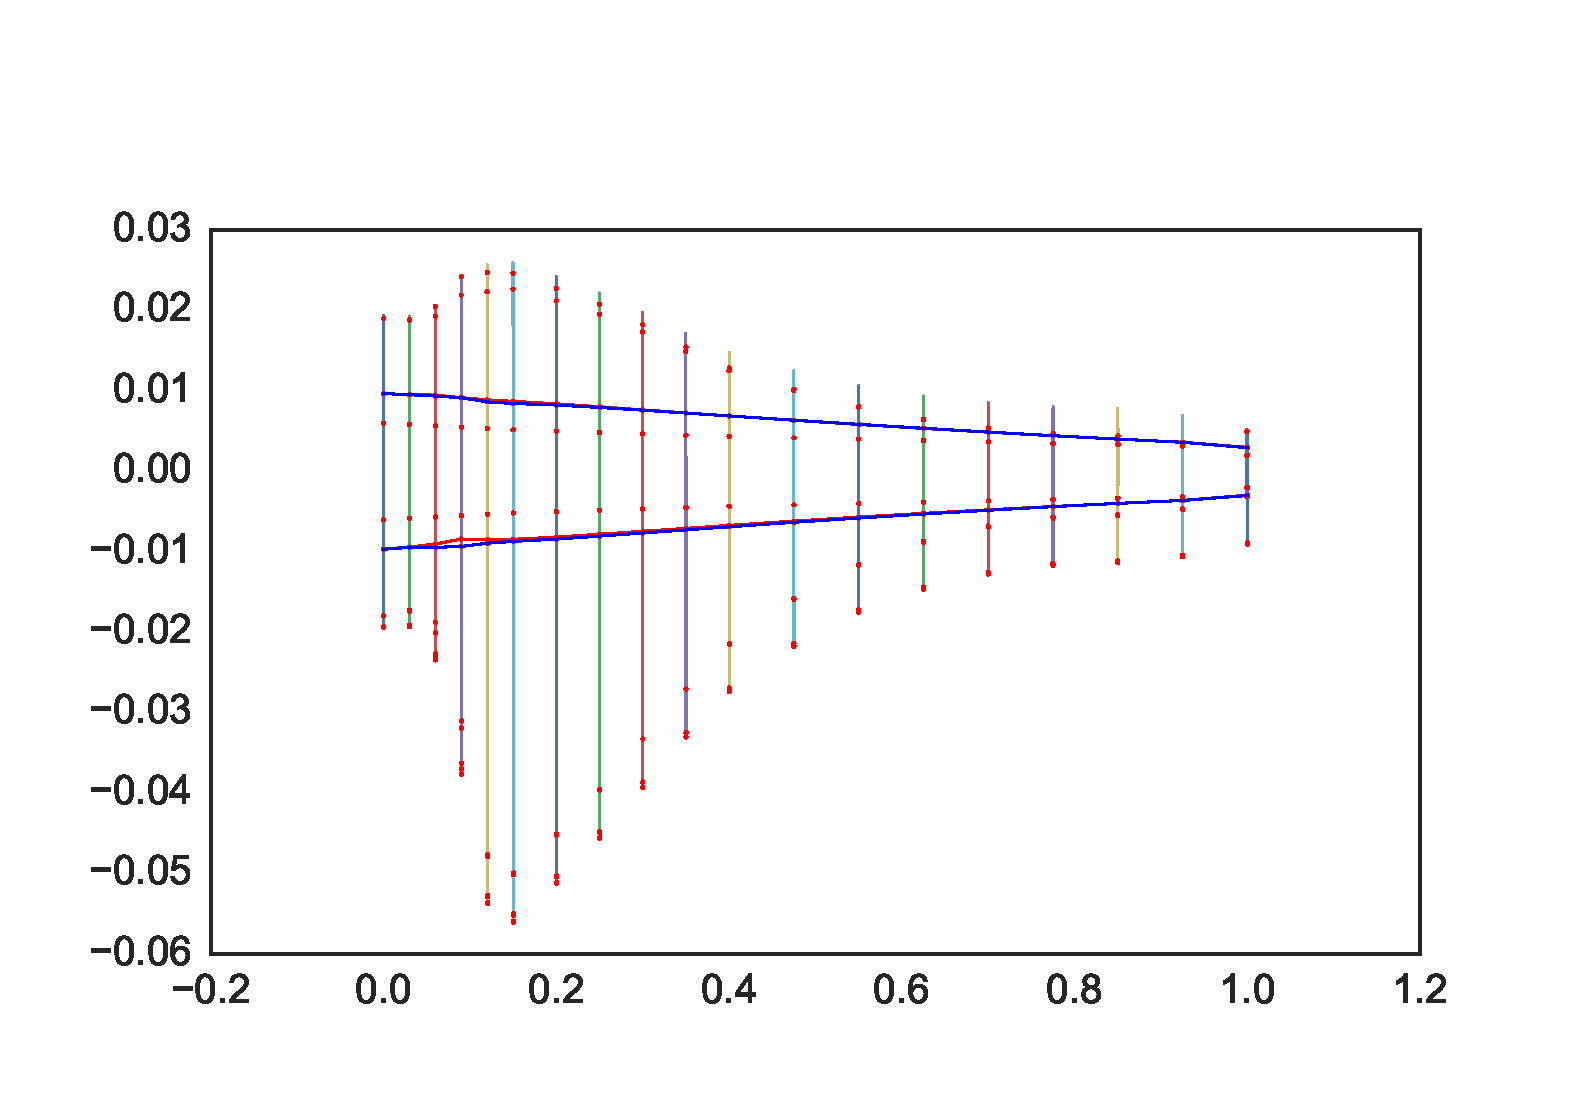
\includegraphics[width=.85\linewidth]{figures/KB1_topview.eps}
\end{center}
\caption{Topview schematic of the KB1 blade structure.}
\label{fig:topview}
\end{figure}

\section{Selected blade design - KB6}
\label{sec:final_design}

\begin{figure}[!ht]
\begin{center}
	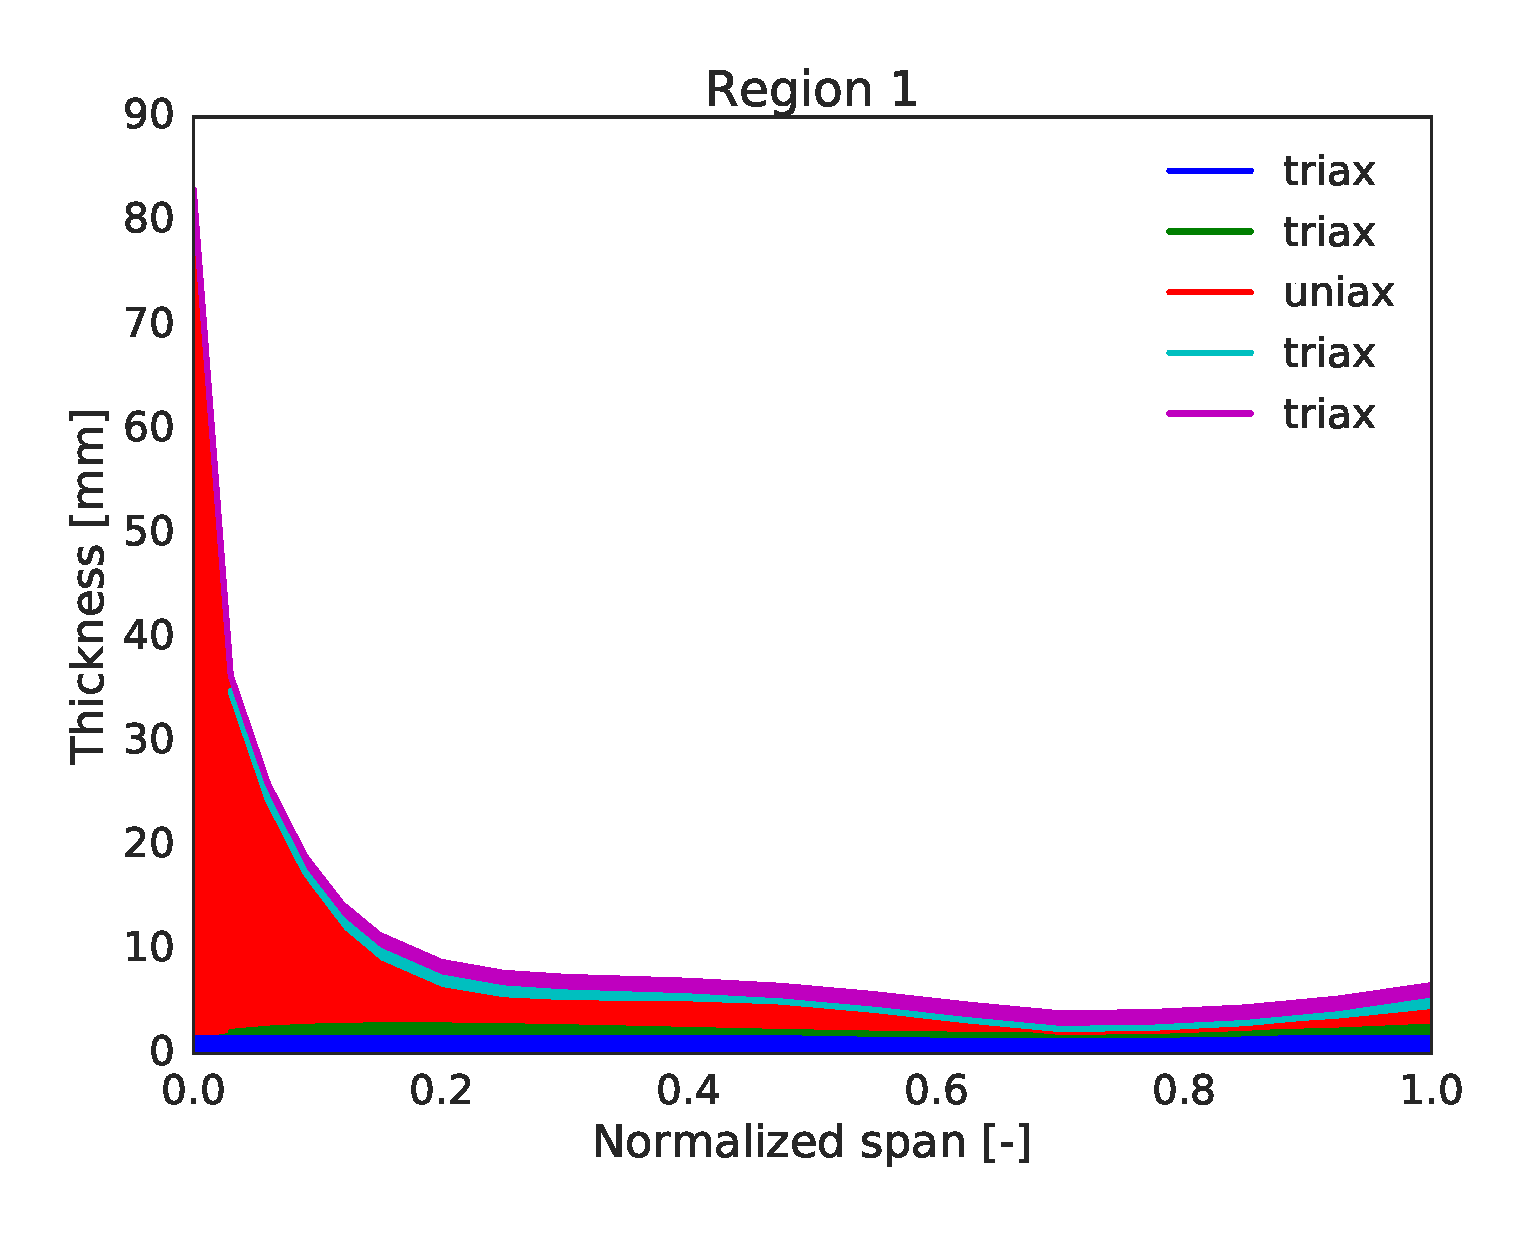
\includegraphics[width=.85\linewidth]{figures/KB6_laminate_layers_r01.eps}
\end{center}
\caption{Material thicknesses in the trailing edge reinforcement of the KB6 blade.}
\label{fig:KB6matstackr01}
\end{figure}

\begin{figure}[!ht]
\begin{center}
	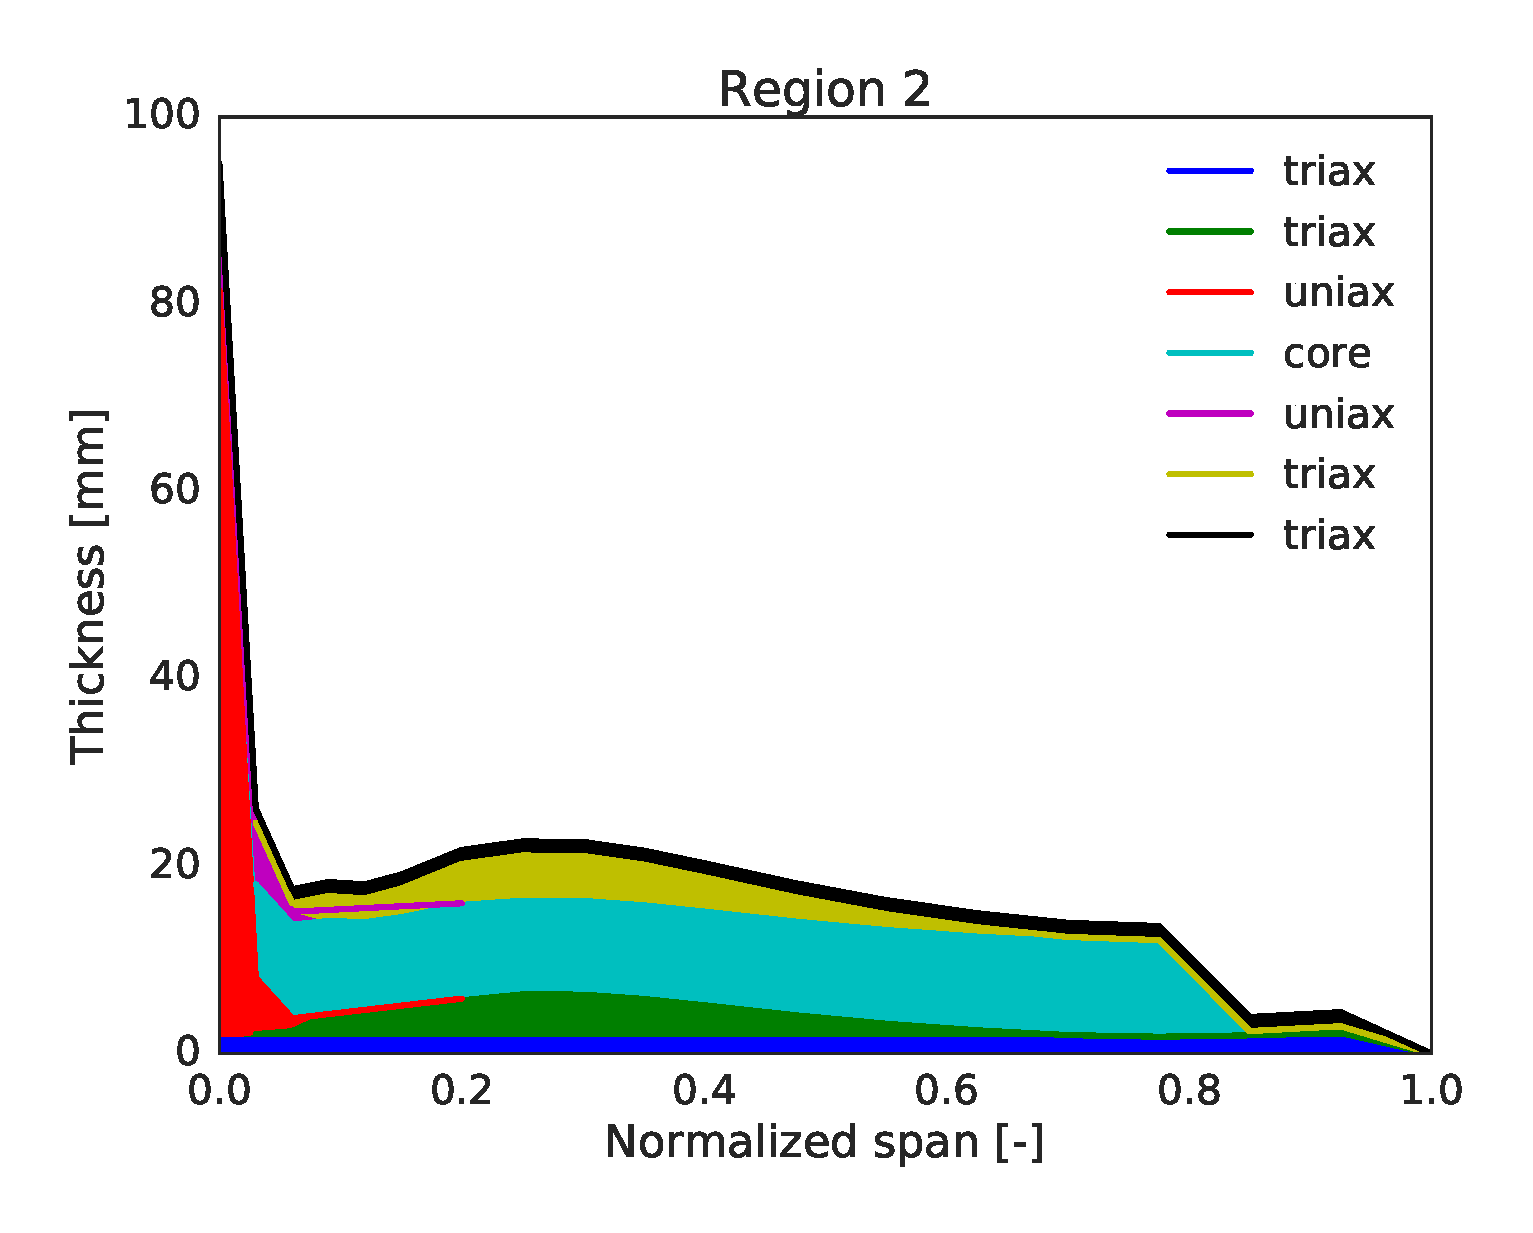
\includegraphics[width=.85\linewidth]{figures/KB6_laminate_layers_r02.eps}
\end{center}
\caption{Material thicknesses in the main panel (immediately behind the spar cap) of the KB6 blade.}
\label{fig:KB6matstackr02}
\end{figure}

\begin{figure}[!ht]
\begin{center}
	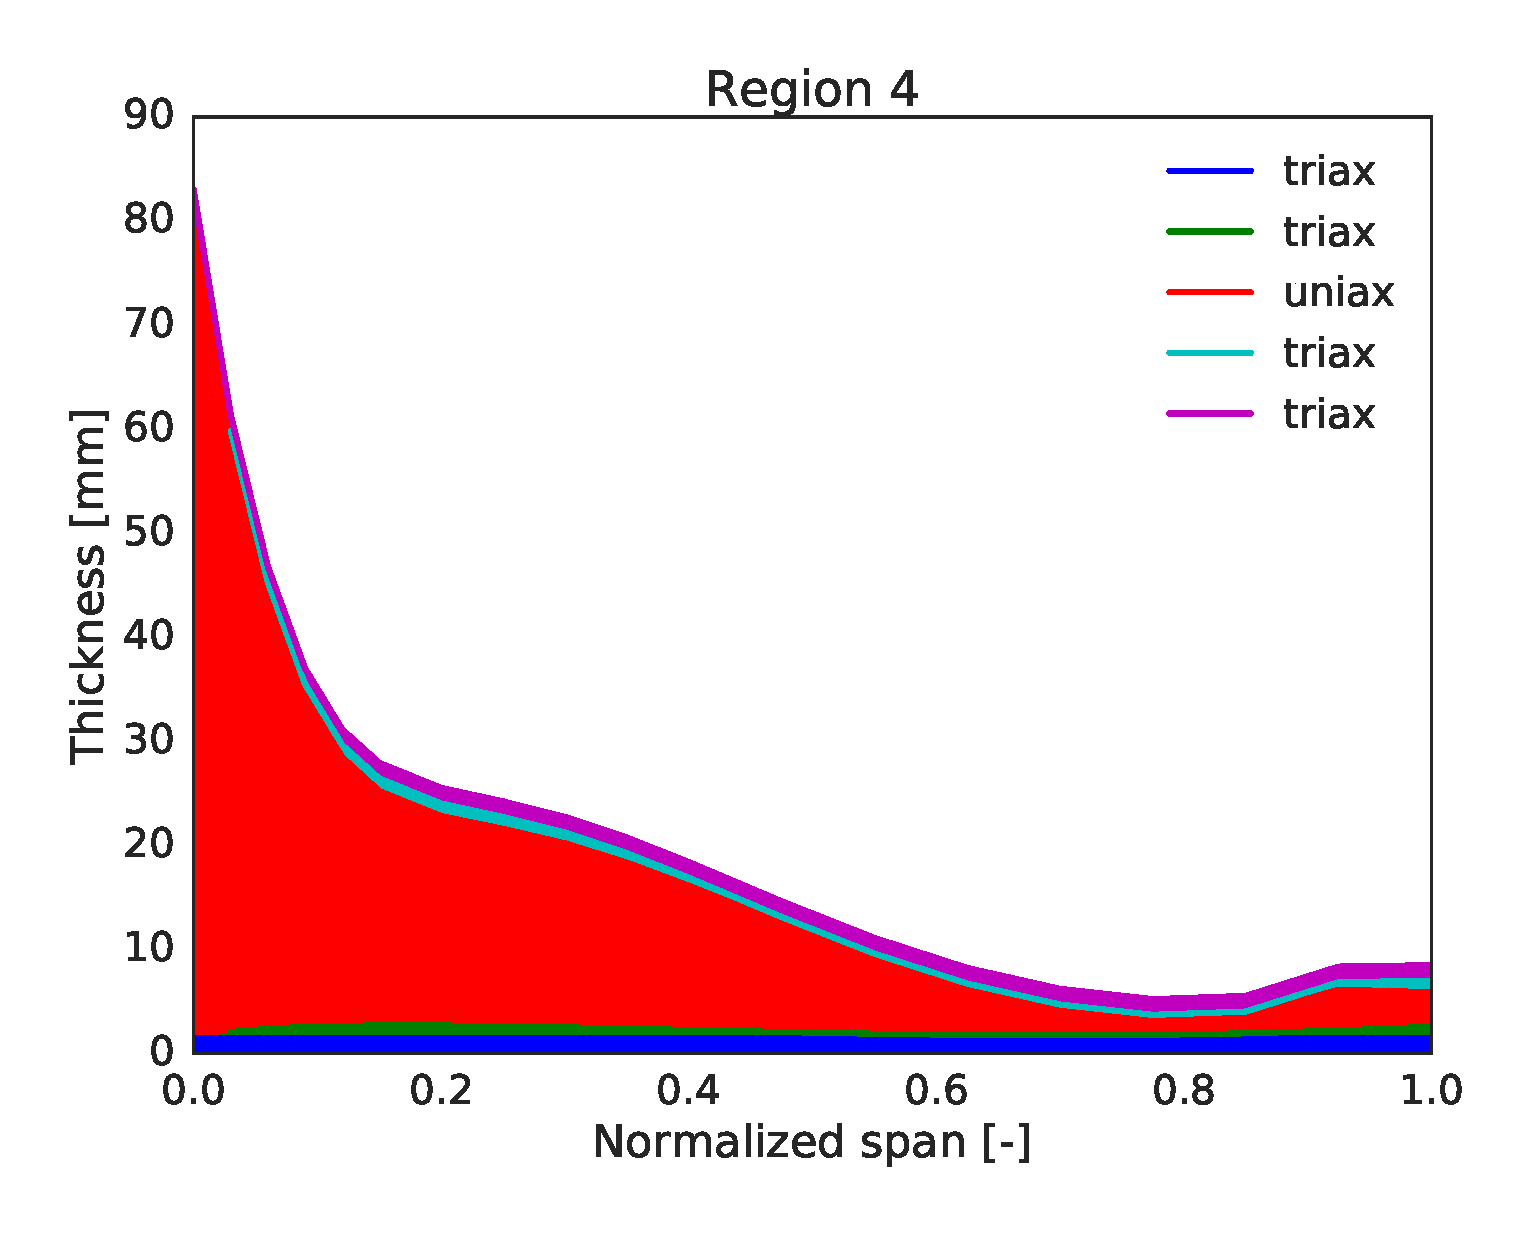
\includegraphics[width=.85\linewidth]{figures/KB6_laminate_layers_r04.eps}
\end{center}
\caption{Material thicknesses in the spar cap of the KB blade.}
\label{fig:KB6matstackr04}
\end{figure}

\begin{figure}[!ht]
\begin{center}
	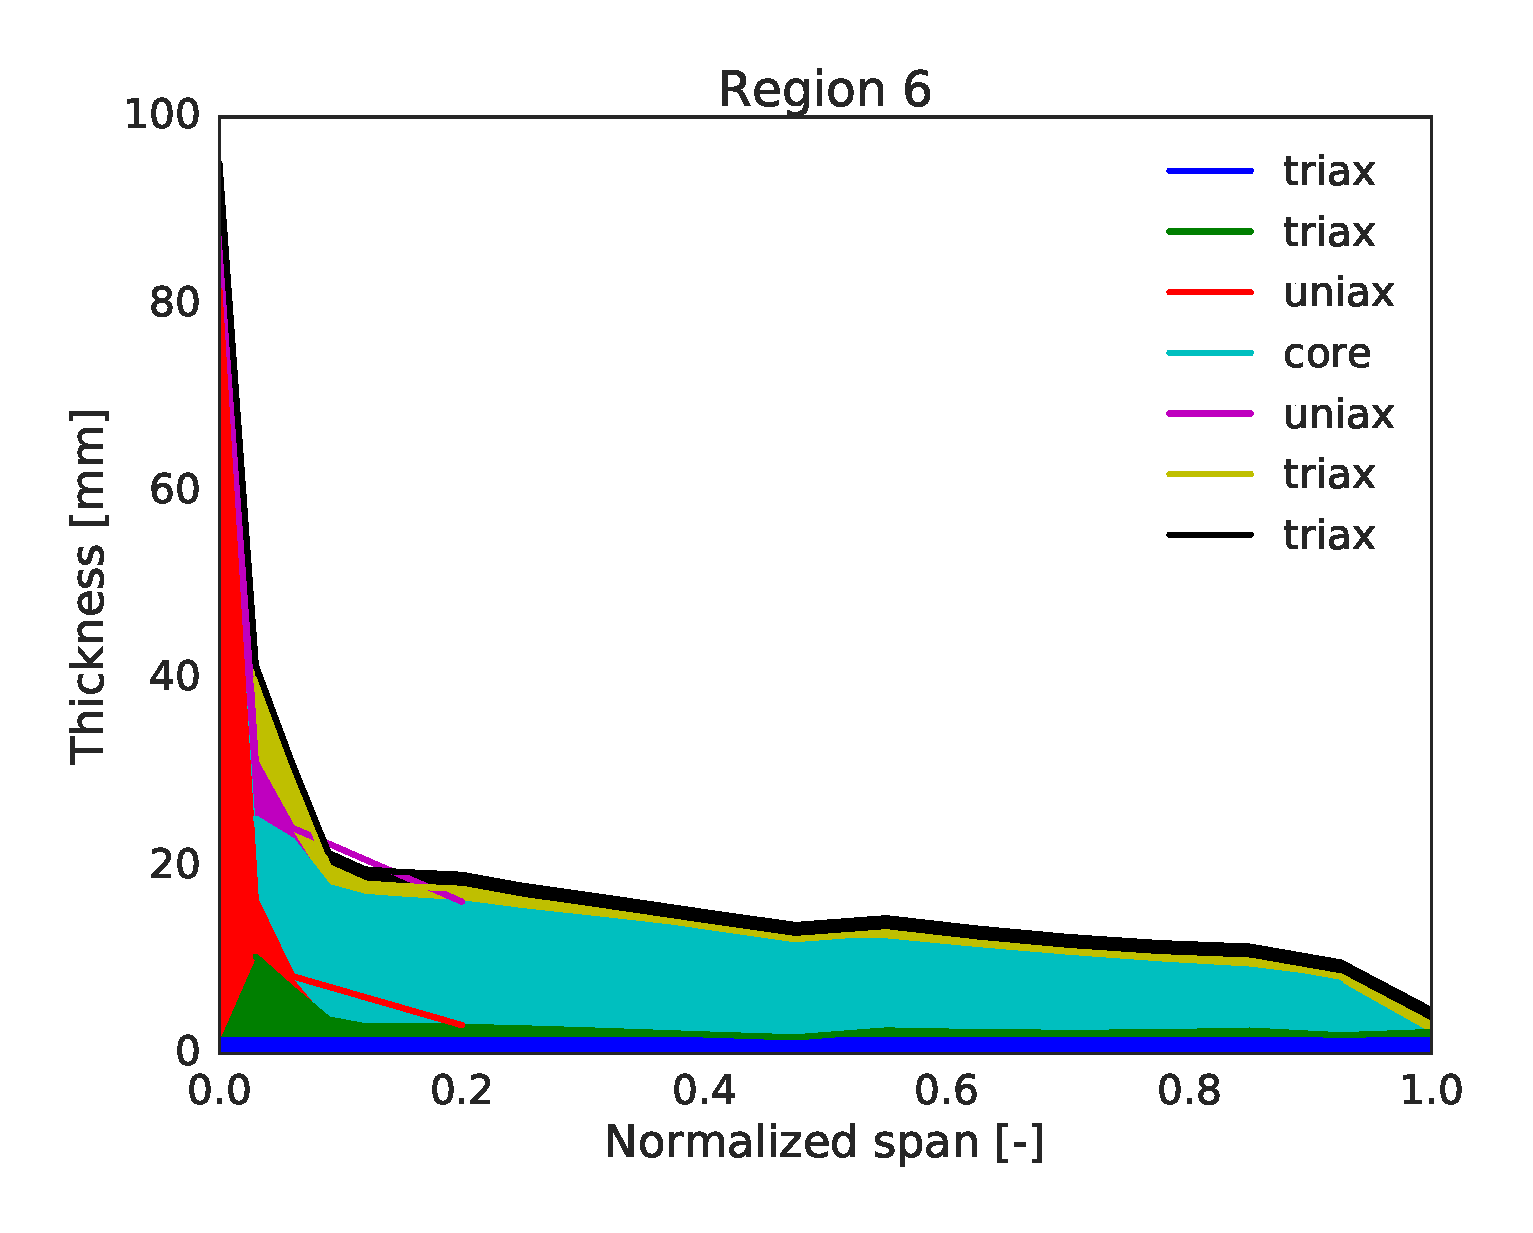
\includegraphics[width=.85\linewidth]{figures/KB6_laminate_layers_r06.eps}
\end{center}
\caption{Material thicknesses in the leading region (immediately in front of the spar cap) of the KB6 blade.}
\label{fig:KB6matstackr06}
\end{figure}

\begin{figure}[!ht]
\begin{center}
	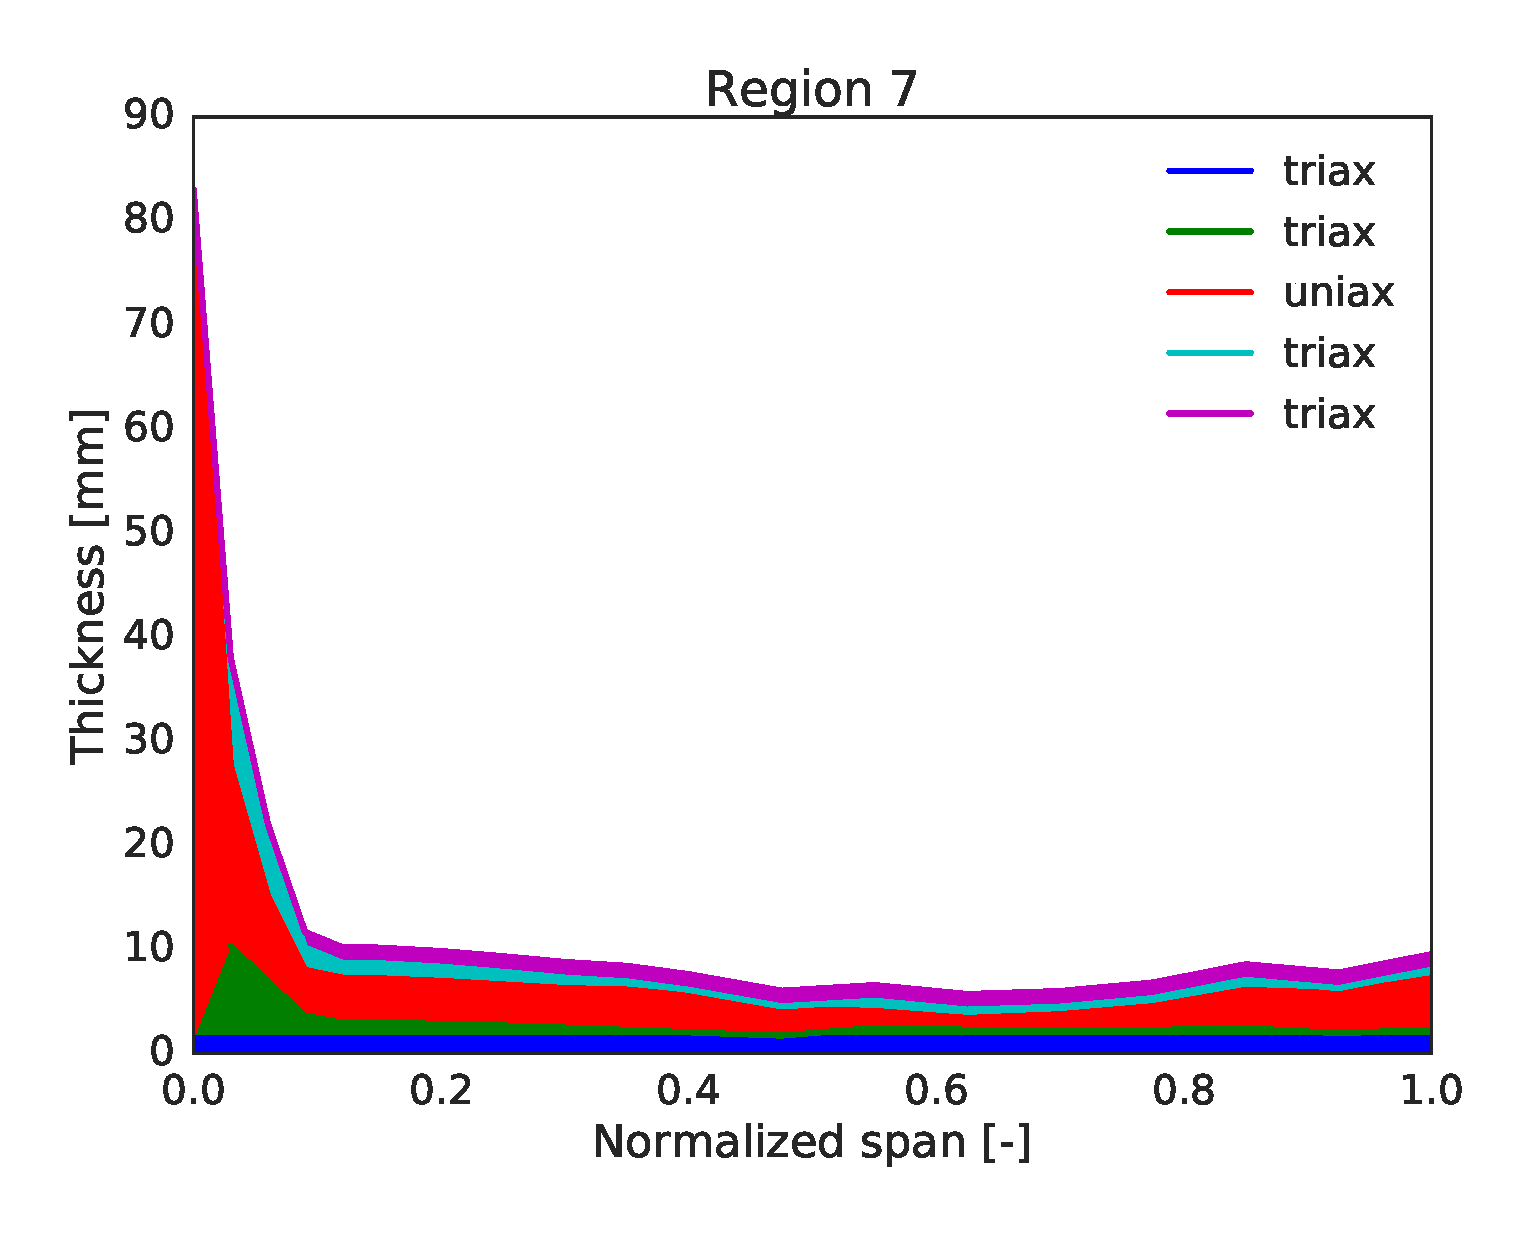
\includegraphics[width=.85\linewidth]{figures/KB6_laminate_layers_r07.eps}
\end{center}
\caption{Material thicknesses in the leading edge reinforcement of the KB6 blade.}
\label{fig:KB6matstackr07}
\end{figure}
%\section{CFD Evaluation of the KB2 Blade}



